% State Of The Art

\chapter{Implementation} % Chapter title

\label{ch:implementation}

%----------------------------------------------------------------------

\section{Statistical variable analysis}
\label{sec:stat-var-analysis}

This section describes the basic properties of each feature we are
using in this particular thesis. Among them we have the count of all
variables, mean, standard deviation, min value, max value, quartiles.
We also add the histogram to have an idea of how the distribution of
the variable works and the boxplot that can help us determine if there
are outliers in the data-set.

There are 27 variables descriptions, three of them are sets of
variables, namely, \textit{Bitcoins Days Destroyed}, which groups 5
individual variables, \textit{Number of Transactions}, that groups 6
individual variables, and \textit{Standard \& Poors 500}, which groups
another 6 individual variables. Therefore in the data-set, every
individual member of said sets, would count as individual feature for
learning purposes.

The data-sets were obtained from a variaty of sources, but mostly from
\href{https://blockchain.info/charts}{blockchain.info}, excluding
\textit{Euro price in USD} that was obtained from the
\href{https://www.ecb.europa.eu/stats/exchange/eurofxref/html/index.en.html}{European
  Central Bank} web site, and the \textit{Standard \& Poors 500} that
was obtained from
\href{https://finance.yahoo.com/q/hp?s=^GSPC\&a=00\&b=3\&c=1950\&d=05\&e=8\&f=2016\&g=d}{Yahoo!
  Finance}.

While all the data-set have daily data points for their values, they
have different spanning dates, been \textit{Euro price in USD} and
\textit{Standard \& Poors 500} that span the most, because they have
more history than Bitcoin. After analyzing the date span of each
variable, we conclude that the interesction of all the sets is in the
range between 03/01/2009 and 28/04/2016.

\subsection{Average Block Size}
\label{sec:avg-block-size}

A concise definition of a block can be found
\href{https://en.bitcoin.it/wiki/Block}{here}: \textit{``Each block
  contains, among other things, a record of some or all recent
  transactions, and a reference to the block that came immediately
  before it. It also contains an answer to a difficult-to-solve
  mathematical puzzle - the answer to which is unique to each
  block.''}

It's clear that, over time, the size of the block is going to
increase, because there are more and more transactions in the Bitcoin
distributed network, due to that
\autoref{fig:avg-block-size-over-time} shows a non-stoppable
increasing.

This variable, called avg-block-size represent the average size of the
blocks in one day measured in MB. One real number data point each day,
at 18:15:05, spanning from 03/01/2009 to 03/05/2016. It was obtained
from the section \textbf{Charts} of
\href{blockchain.info}{blockchain.info}

\begin{figure}[bth]
  \myfloatalign
  {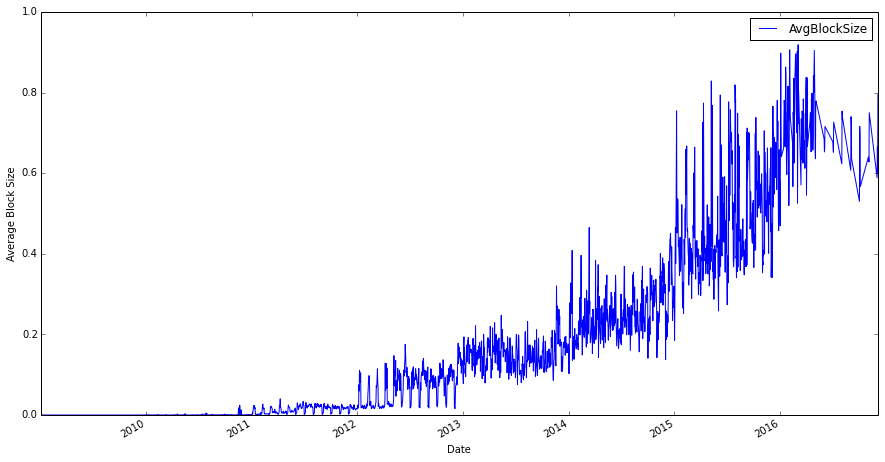
\includegraphics[width=1\linewidth]
    {gfx/avg-block-size-over-time}} 
  \caption{Average Block Size Over Time}
  \label{fig:avg-block-size-over-time}
\end{figure}

In \autoref{fig:avg-block-size-over-time} can be seen how the average
block size has been increasing since the creation of Bitcoin. In 2015
the average block started to dangerously approach the limit of 1 MB,
which is causing a big debate in the Bitcoin community whether they
should increase this limit or not.

\begin{figure}[bth]
  \myfloatalign
  {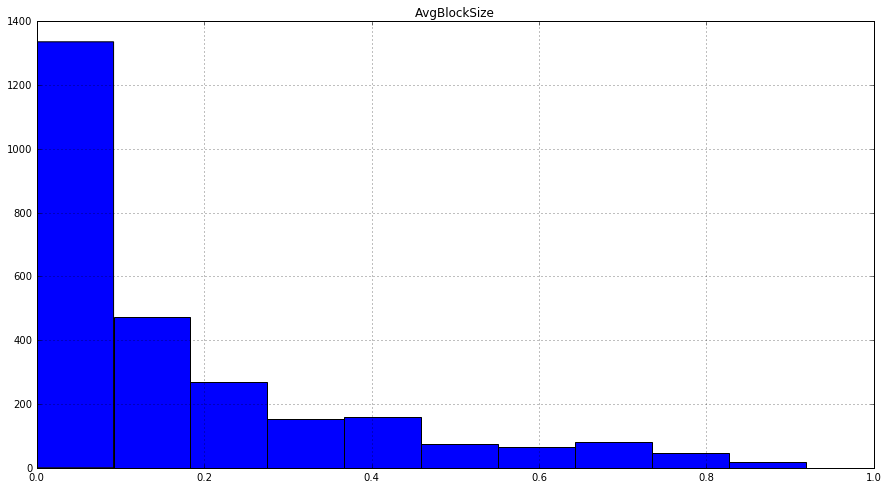
\includegraphics[width=1\linewidth]
    {gfx/avg-block-size-histogram}} 
  \caption{Average Block Size Histogram}
  \label{fig:avg-block-size-histogram}
\end{figure}

\begin{table}
  \myfloatalign
  \small
  \begin{tabularx}{\textwidth}{XX} 
    \toprule
    \tableheadline{Measure} & \tableheadline{Value} \\
    \midrule 
    count  & $2678$\\
    mean   & $0.165$\\
    median & $0.092$\\
    std    & $0.209$\\
    min    & $0.000$\\
    $25$\% & $0.000$\\
    $50$\% & $0.092$\\
    $75$\% & $0.242$\\
    max    & $0.918$\\
    \bottomrule
  \end{tabularx}
  \caption{Statistical values for 
    \textit{Average Block Size}}
  \label{tab:stats-avg-block-size}
\end{table}

\begin{figure}[bth]
  \myfloatalign
    {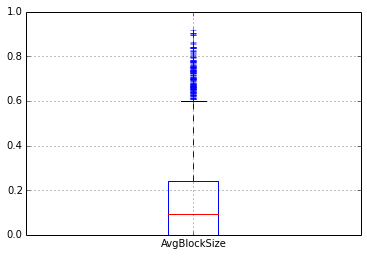
\includegraphics[width=1\linewidth]
      {gfx/avg-block-size-boxplot}}               
    \caption{Average Block Size Boxplot}
    \label{fig:avg-block-size-boxplot}
\end{figure}

\clearpage

%----------------------------------------------------------------------

\subsection{Bitcoin Days Destroyed}
\label{sec:bitcoin-days-destroyed}

\begin{figure}[bth]
  \myfloatalign
  {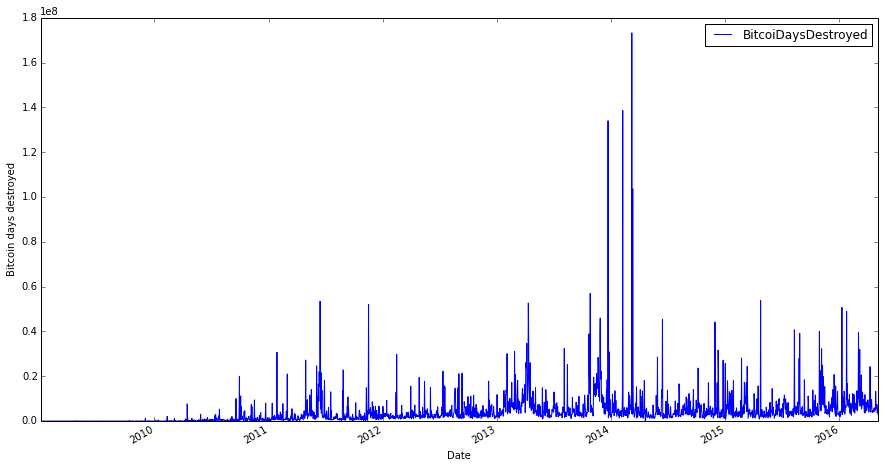
\includegraphics[width=1\linewidth]
    {gfx/bitcoin-days-destroyed-over-time}}
  \caption{Bitcoin Days Destroyed Over Time}
  \label{fig:bitcoin-days-destroyed-over-time}
\end{figure}

\begin{figure}[bth]
  \myfloatalign
  {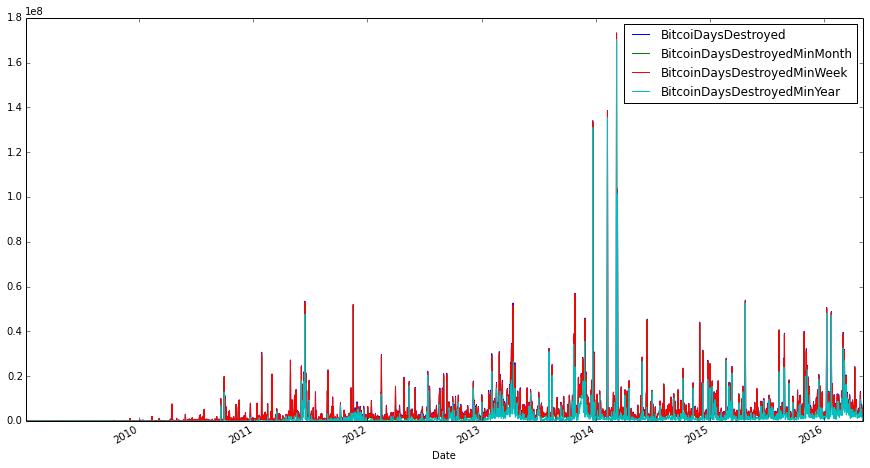
\includegraphics[width=1\linewidth]
    {gfx/bitcoin-days-destroyed-over-time-rest}}
  \caption{Bitcoin Days Destroyed Over Time without Cumulative}
  \label{fig:bitcoin-days-destroyed-over-time-rest}
\end{figure}

Bitcoin Days Destroyed is a weighted measure of aggregate economic
activity, placing value on transacted coins in proportion to the time
they have spent idle on the Bitcoin blockchain. For any given
transaction, Days Destroyed is calculated by multiplying its estimated
transaction value by the number of days since the coins within the
transaction were last spent. Bitcoin Days Destroyed is a useful proxy
for measuring growth in real value transacted on the Bitcoin
blockchain over time, since it controls for rapid movement of coins
between wallets (potentially owned by just one entity). One integer
data point each day, at 18:15:05, spanning from 03/01/2009 to
03/05/2016.

In \autoref{fig:bitcoin-days-destroyed-over-time} we shows data over
time for Bitcoin Days Destroyed, Bitcoin Days Destroyed Min Month,
Bitcoin Days Destroyed Min Week, Bitcoin Days Destroyed Min Year and
Bitcoin Days Destroyed Cumulative. Due to scaling issues, we printed
\autoref{fig:bitcoin-days-destroyed-over-time-rest} without Bitcoin
Days Destroyed Cumulative in order to be able to see how the rest of
the variables fluctuate.

To better understand this set of variable we include a quote extracted
from
\href{http://bitcoin.stackexchange.com/questions/845/what-are-bitcoin-days-destroyed}{Bitcoin
  Beta | Stack Exchange}:

``\textit{The idea of "bitcoin days destroyed" came about because it
  was realized that total transaction volume per day might be an
  inappropriate measure of the level of economic activity in Bitcoin.
  After all, someone could be sending the same money back and forth
  between their own addresses repeatedly. If you sent the same 50 btc
  back and forth 20 times, it would look like 1000 btc worth of
  activity, while in fact it represents almost nothing in terms of
  real transaction volume.}

\textit{With "bitcoin days destroyed", the idea is instead to give
  more weight to coins which haven't been spent in a while. To do
  this, you multiply the amount of each transaction by the number of
  days since those coins were last spent. So, 1 bitcoin that hasn't
  been spent in 100 days (1 bitcoin * 100 days) counts as much as 100
  bitcoins that were just spent yesterday (100 bitcoins * 1 day).
  Because you can think of these "bitcoin days" as building up over
  time until a transaction actually occurs, the actual measure is
  called "bitcoin days destroyed". This is believed to give a better
  indication of how much real economic activity is occurring on the
  bitcoin network.}

\textit{ So how well does it work? Well, it's still not perfect,
  because the other day I moved some coins out of a wallet they've
  been in for several months without spending them or giving them
  away. And some genuine businesses have very rapid turnover in
  bitcoins, so they're not being measured well by this method. But it
  does do a good job of filtering out the "noise" of bitcoins that are
  just "bouncing around" without really going anywhere. The graph of
  overall bitcoin days destroyed is believed to show that the genuine
  level of activity in the Bitcoin economy is continually
  increasing--it's not just one person experimenting by rapidly
  sending the same coins back and forth, flooding the network with
  meaningless chatter. Looks pretty good, hey?}''

\begin{table}
  \myfloatalign
  \tiny
  \begin{tabularx}{\textwidth}{XXXXXX} 
    \toprule
    \tableheadline{Measure} & \tableheadline{DaysDestroyed} &
    \tableheadline{Cumulative} &
    \tableheadline{MinMonth} &
    \tableheadline{MinWeek} &
    \tableheadline{MinYear} \\
    \midrule 
    count  & $2.679e+03$ & $2.679e+03$ & $2.679e+03$ & $2.679e+03$ & $2.679e+03$ \\
    median & $2.456e+06$ & $2.265e+09$ & $1.868e+06$ & $2.210e+06$ & $4.164e+05$ \\
    mean   & $4.146e+06$ & $3.609e+09$ & $3.649e+06$ & $3.947e+06$ & $1.774e+06$ \\
    std    & $7.778e+06$ & $3.572e+09$ & $7.629e+06$ & $7.721e+06$ & $6.404e+06$ \\
    min    & $0$         & $0$         & $0$         & $0$         & $0$         \\
    $25$\  & $5.017e+05$ & $1.817e+08$ & $3.028e+05$ & $4.384e+05$ & $0$         \\
    $50$\  & $2.456e+06$ & $2.265e+09$ & $1.868e+06$ & $2.210e+06$ & $4.164e+05$ \\
    $75$\  & $4.745e+06$ & $6.971e+09$ & $4.001e+06$ & $4.454e+06$ & $1.568e+06$ \\
    max    & $1.732e+08$ & $1.110e+10$ & $1.727e+08$ & $1.730e+08$ & $1.702e+08$ \\
    \bottomrule
  \end{tabularx}
  \caption{Statistical values for \textit{Bitcoin Days Destroyed}}
  \label{tab:bitcoin-days-destroyed}
\end{table}

\begin{figure}[bth]
  \myfloatalign
  {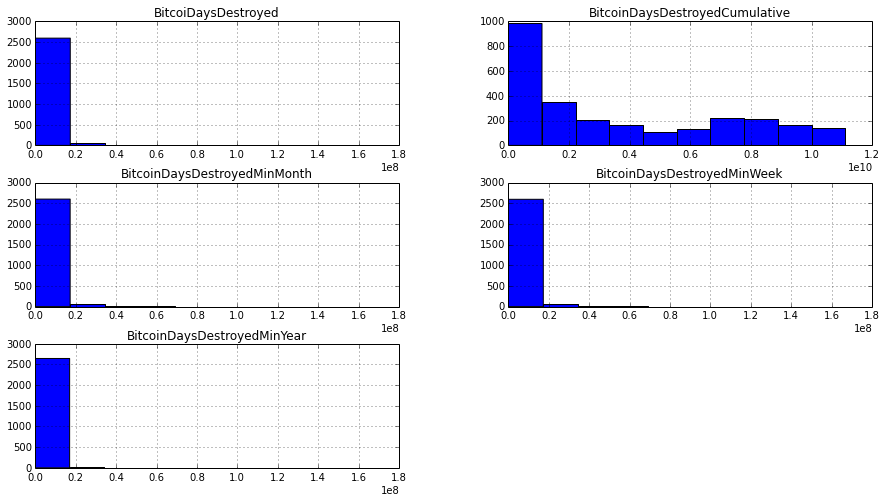
\includegraphics[width=1\linewidth]
    {gfx/bitcoin-days-destroyed-histogram}}
  \caption{Bitcoin Days Destroyed Histogram}
  \label{fig:bitcoin-days-destroyed-histogram}
\end{figure}

\begin{figure}[bth]
  \myfloatalign
  {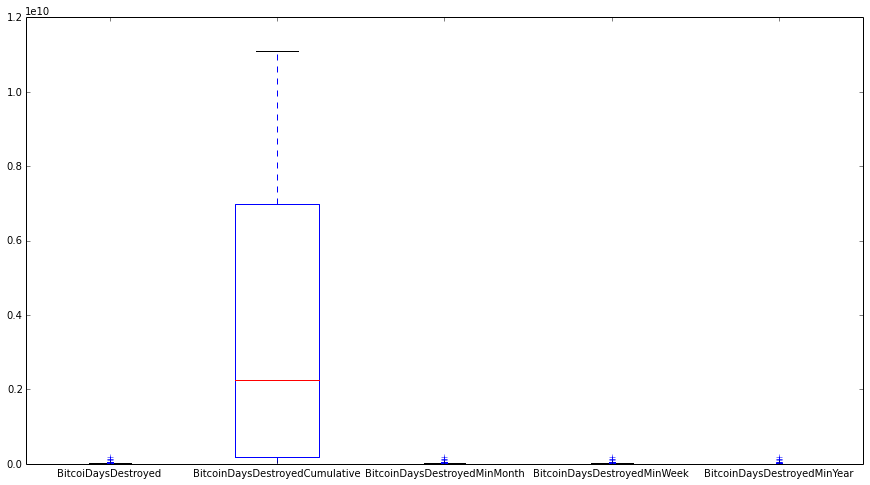
\includegraphics[width=1\linewidth]
    {gfx/bitcoin-days-destroyed-boxplot}}
  \caption{Bitcoin Days Destroyed Boxplot}
  \label{fig:bitcoin-days-destroyed-boxplot}
\end{figure}

\begin{figure}[bth]
  \myfloatalign
  {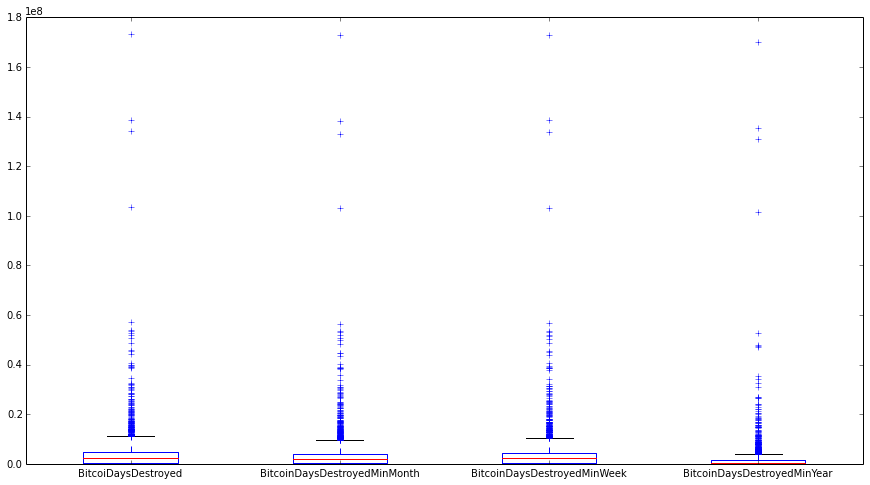
\includegraphics[width=1\linewidth]
    {gfx/bitcoin-days-destroyed-boxplot-rest}}
  \caption{Bitcoin Days Destroyed Boxplot Without Cumulative}
  \label{fig:bitcoin-days-destroyed-boxplot-rest}
\end{figure}

\clearpage

%----------------------------------------------------------------------

\subsection{Block Size}
\label{sec:block-size}

\begin{figure}[bth]
  \myfloatalign
  {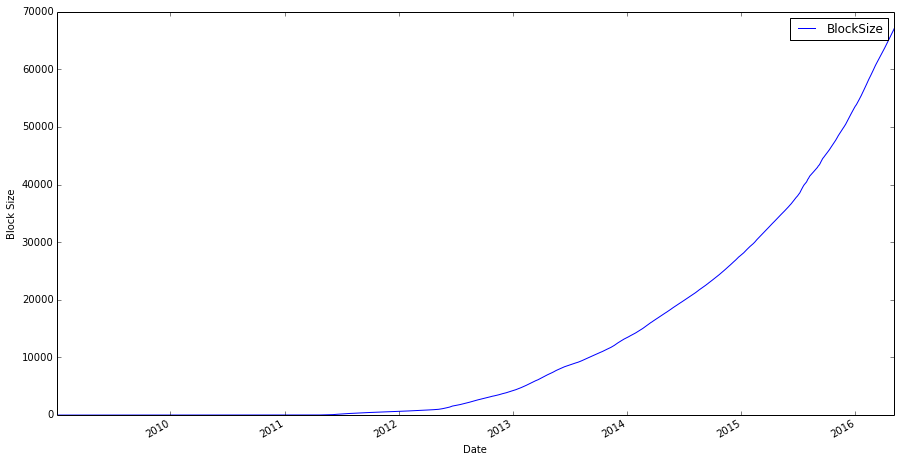
\includegraphics[width=1\linewidth]
    {gfx/block-size-over-time}}
  \caption{Block Size Over Time}
  \label{fig:block-size-over-time}
\end{figure}

The total size (in MB) of all block headers and transactions. Not
including database indexes. One real number data point each day, at
18:15:05, spanning from 03/01/2009 to 03/05/2016.

The total block size is increasing exponentialy as seen in
\autoref{fig:block-size-over-time}. This basically represents that the
total ammount of transactions are increasing at that rate.

\begin{table}
  \myfloatalign
  %\small
  \begin{tabularx}{\textwidth}{XX} 
    \toprule
    \tableheadline{Measure} & \tableheadline{Value} \\
    \midrule 
    count  & $2678$   \\
    mean   & $9.727$  \\
    median & $6.219$  \\
    std    & $13.268$ \\
    min    & $0$      \\
    25\%   & $1.301$  \\
    50\%   & $6.219$  \\
    75\%   & $10.401$ \\
    max    & $90.202$ \\
    \bottomrule
  \end{tabularx}
  \caption{Statistical values for \textit{Block Size}}
  \label{tab:block-size}
\end{table}

\begin{figure}[bth]
  \myfloatalign
  {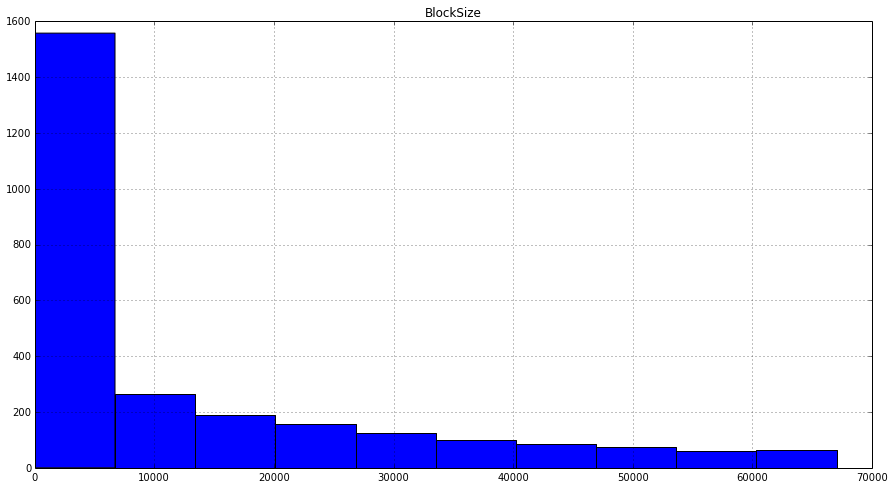
\includegraphics[width=1\linewidth]
    {gfx/block-size-histogram}}
  \caption{Block Size Histogram}
  \label{fig:block-size-histogram}
\end{figure}

\begin{figure}[bth]
  \myfloatalign
  {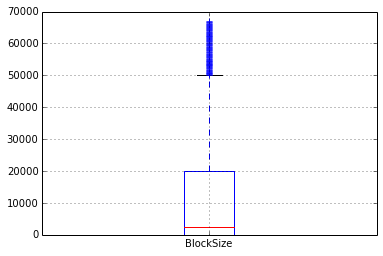
\includegraphics[width=1\linewidth]
    {gfx/block-size-boxplot}}
  \caption{Block Size Boxplot}
  \label{fig:block-size-boxplot}
\end{figure}

\clearpage
%----------------------------------------------------------------------

\subsection{Cost Per Transaction}
\label{sec:cost-per-transaction}

This variable shows miners revenue (in USD) divided by the number of
transactions. Miners revenue are a result of the transaction fees plus
the reward for block discovery. The block discovery reward is fixed by
the community, is up to the miner to accept any transaction regardless
of the fee in the transaction. A miner can choose not to add any
transaction at all to the block, or add transactions with a $0$
BTC fee.

\autoref{fig:cost-per-transaction-over-time} shows that in the end of
2010 the Cost Per Transactions started to increase and had a local
maximum followed by another local maximum in mid 2011. This two peaks
took place in a low price of Bitcoin scenario, hence probably the
blocks were introduced with a small amount of transactions, and with a
subtle increase in the Bitcoin price the ratio would increase.

On the contrary, the two peaks of 2014 are in the highest price of the
Bitcoin history, where the number of transactions would make little
effect. The median transactions per block is $205$
(\autoref{tab:n-transactions-per-block}), while the price in that
period fluctuates between $700$
USD and $1100$
USD approximately. It can be noticed in
\autoref{fig:miners-revenue-over-time} that miners made a revenue of
$5000000$
USD in one peak and $3000000$
USD in the other peak, and
\autoref{fig:n-transactions-multiple-over-time} indicates that at the
same time, the number of transactions were $100000$ for both peaks.

\begin{figure}[bth]
  \myfloatalign
  {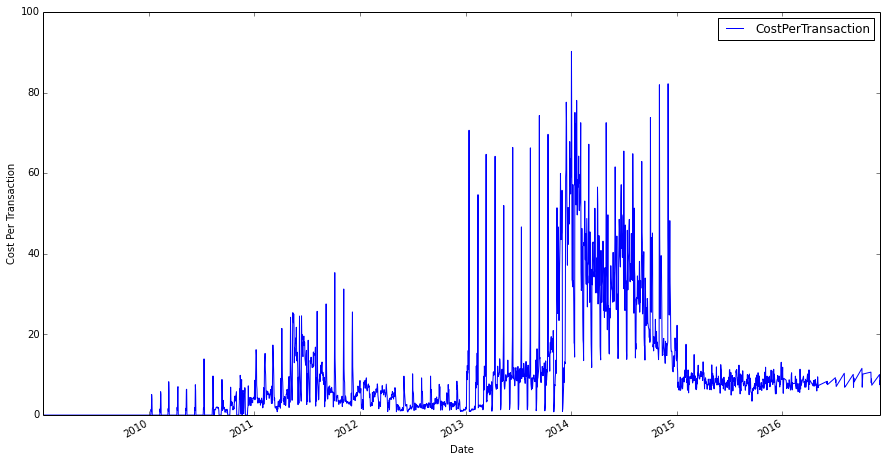
\includegraphics[width=1\linewidth]
    {gfx/cost-per-transaction-over-time}}
  \caption{Cost Per Transaction Over Time}
  \label{fig:cost-per-transaction-over-time}
\end{figure}

The dataset comprises one real number data point each day, at
18:15:05, spanning from 03/01/2009 to 03/05/2016.

\begin{table}
  \myfloatalign
  %\small
  \begin{tabularx}{\textwidth}{XX} 
    \toprule
    \tableheadline{Measure} & \tableheadline{Value} \\
    \midrule 
    count  & $2678$   \\
    mean   & $9.727$  \\
    median & $6.219$  \\
    std    & $13.268$ \\
    min    & $0$      \\
    $25$\  & $1.301$  \\
    $50$\  & $6.219$  \\
    $75$\  & $10.401$ \\
    max    & $90.202$ \\
    \bottomrule
  \end{tabularx}
  \caption{Statistical values for \textit{Cost Per Transaction}}
  \label{tab:cost-per-transaction}
\end{table}

\begin{figure}[bth]
  \myfloatalign
  {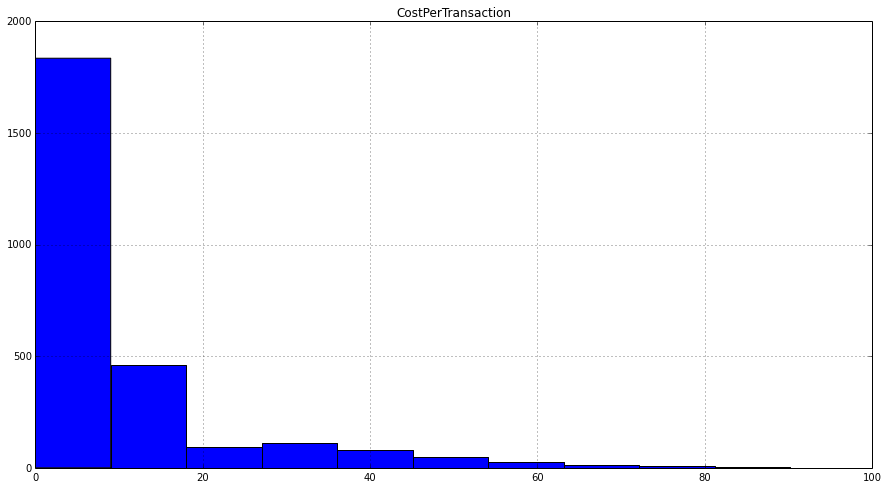
\includegraphics[width=1\linewidth]
    {gfx/cost-per-transaction-histogram}}
  \caption{Cost Per Transaction Histogram}
  \label{fig:cost-per-transaction-histogram}
\end{figure}

\begin{figure}[bth]
  \myfloatalign
  {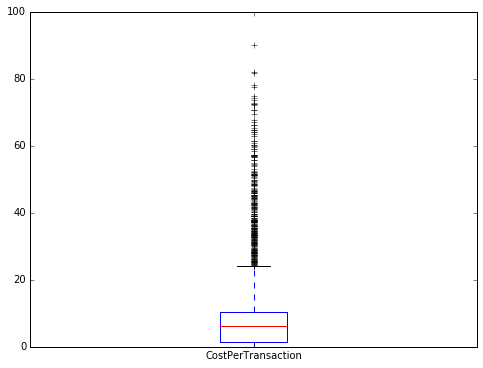
\includegraphics[width=1\linewidth]
    {gfx/cost-per-transaction-boxplot}}
  \caption{Cost Per Transaction Boxplot}
  \label{fig:cost-per-transaction-boxplot}
\end{figure}

\clearpage
%----------------------------------------------------------------------

\subsection{Cost Per Transaction Percent}
\label{sec:cost-per-transaction-percent}

\begin{figure}[bth]
  \myfloatalign
  {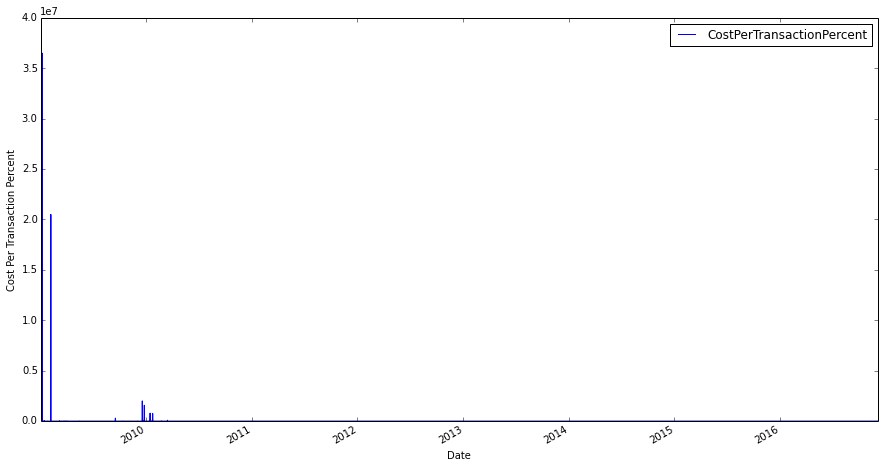
\includegraphics[width=1\linewidth]
    {gfx/cost-per-transaction-percent-over-time}}
  \caption{Cost Per Transaction Percent Over Time}
  \label{fig:cost-per-transaction-percent-over-time}
\end{figure}

This variable shows miners revenue as percentage of the transaction
volume. Basically what
\autoref{fig:cost-per-transaction-percent-over-time} shows is that
over time, the miners revenue is decreasing with respect to the
transaction amount itself.

The dataset comprises one real number data point each day, at
18:15:05, spanning from 03/01/2009 to 03/05/2016.

\begin{table}
  \myfloatalign
  %\small
  \begin{tabularx}{\textwidth}{XX} 
    \toprule
    \tableheadline{Measure} & \tableheadline{Value} \\
    \midrule 
    count  & $2678$       \\
    mean   & $23603.541$  \\
    median & $3.283$      \\
    std    & $810554.930$ \\
    min    & $0$          \\
    25\%   & $1.580$      \\
    50\%   & $3.283$      \\
    75\%   & $9.606$      \\
    max    & $36500000$   \\
    \bottomrule
  \end{tabularx}
  \caption{Statistical values for \textit{Cost Per Transaction Percent}}
  \label{tab:cost-per-transaction-percent}
\end{table}

\begin{figure}[bth]
  \myfloatalign
  {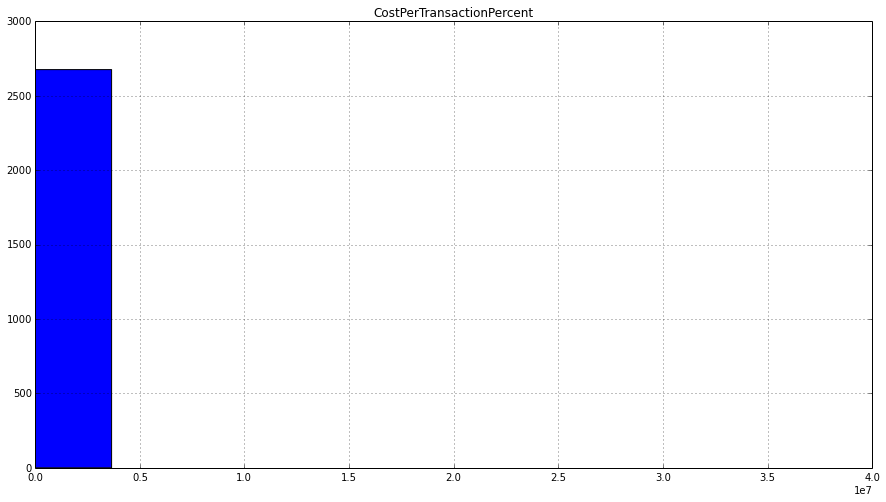
\includegraphics[width=1\linewidth]
    {gfx/cost-per-transaction-percent-histogram}}
  \caption{Cost Per Transaction Percent Histogram}
  \label{fig:cost-per-transaction-percent-histogram}
\end{figure}

\begin{figure}[bth]
  \myfloatalign
  {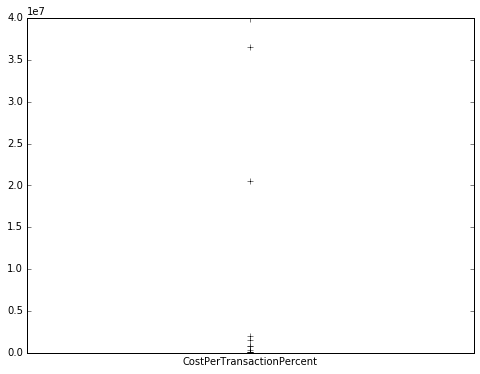
\includegraphics[width=1\linewidth]
    {gfx/cost-per-transaction-percent-boxplot}}
  \caption{Cost Per Transaction Percent Boxplot}
  \label{fig:cost-per-transaction-percent-boxplot}
\end{figure}

\clearpage
%----------------------------------------------------------------------

\subsection{Difficulty}
\label{sec:difficulty}

\begin{figure}[bth]
  \myfloatalign
  {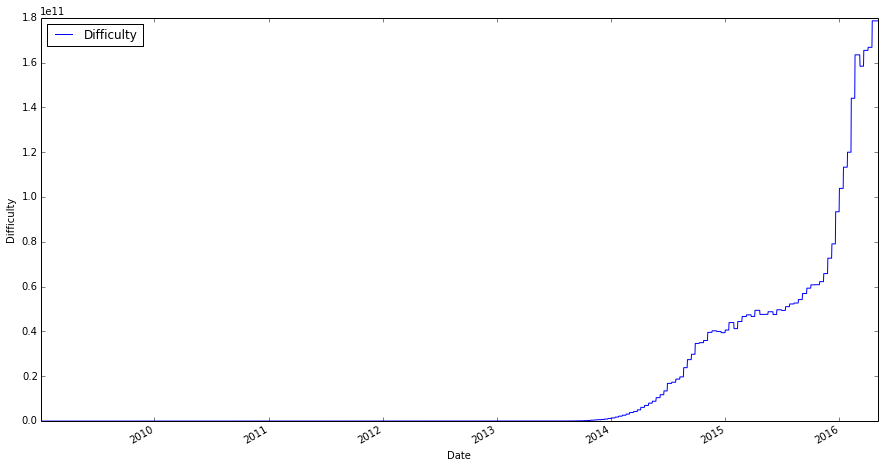
\includegraphics[width=1\linewidth]
    {gfx/difficulty-over-time}}
  \caption{Difficulty Over Time}
  \label{fig:difficulty-over-time}
\end{figure}

A relative measure of how difficult it is to find a new block. The
difficulty is adjusted periodically as a function of how much hashing
power has been deployed by the network of miners. That can be seen
looking at how similar are \autoref{fig:difficulty-over-time} and
\autoref{fig:hash-rate-over-time}. The graphic representing the
difficulty has a discrete shape, that is because the difficulty is
adjusted automatically every 2016 blocks, and changes equally for the
entire Bitcoin network. Until 2014, the difficulty of mining was
very low, it started to raise probably because the trade volume in the
end of 2013 and start of 2014 was approximately 70.000.000\$, which
attracted professional miners with a greater processing power, those
creating more and more blocks and augmenting the difficulty of mining.

The dataset comprises one real number data point each day, at
18:15:05, spanning from 03/01/2009 to 03/05/2016.

\begin{table}
  \myfloatalign
  %\small
  \begin{tabularx}{\textwidth}{XX} 
    \toprule
    \tableheadline{Measure} & \tableheadline{Value} \\
    \midrule 
    count  & $2.678e+03$   \\
    mean   & $1.683e+10$   \\
    median & $2440642.606$ \\
    std    & $3.561e+10$   \\
    min    & $0$           \\
    25\%   & $3.091e+03$   \\
    50\%   & $2.440e+06$   \\
    75\%   & $1.681e+10$   \\
    max    & $1.786e+11$   \\
    \bottomrule
  \end{tabularx}
  \caption{Statistical values for \textit{Difficulty}}
  \label{tab:difficulty}
\end{table}

\begin{figure}[bth]
  \myfloatalign
  {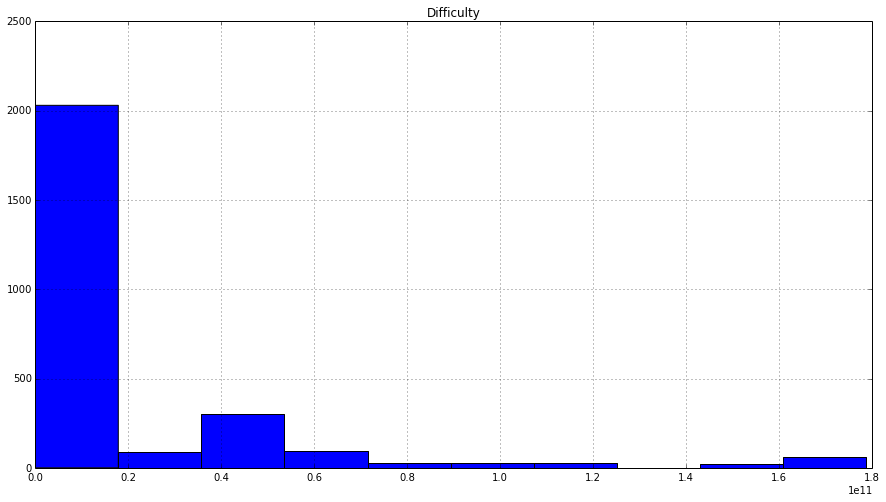
\includegraphics[width=1\linewidth]
    {gfx/difficulty-histogram}}
  \caption{Difficulty Histogram}
  \label{fig:difficulty-histogram}
\end{figure}

\begin{figure}[bth]
  \myfloatalign
  {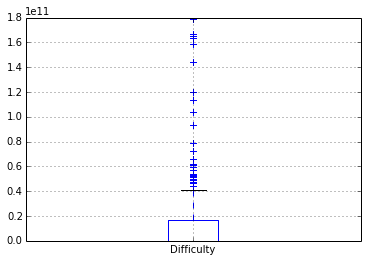
\includegraphics[width=1\linewidth]
    {gfx/difficulty-boxplot}}
  \caption{Difficulty Boxplot}
  \label{fig:difficulty-boxplot}
\end{figure}

\clearpage
%----------------------------------------------------------------------

\subsection{Estimated Transaction Volume}
\label{sec:estimated-transaction-volume}

\begin{figure}[bth]
  \myfloatalign
  {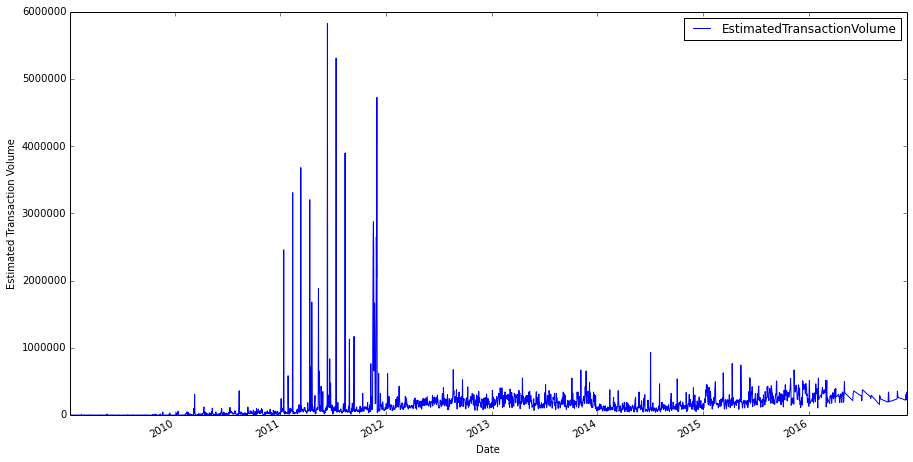
\includegraphics[width=1\linewidth]
    {gfx/estimated-transaction-volume-over-time}}
  \caption{Estimated Transaction Volume Over Time}
  \label{fig:estimated-transaction-volume-over-time}
\end{figure}

The total estimated value of transactions on the Bitcoin blockchain
(does not include coins returned to sender as change). The transaction
volume represented in
\autoref{fig:estimated-transaction-volume-over-time} is very slowly
increasing, meaning that more transactions in Bitcoin are processed.
However, it doesn't represent the actual value of transactions,
because people think in their local currency when trading or shopping,
and Bitcoin's value is volatile. The next variable, \textit{Estimated
  Transaction Volume USD}, is more useful because it gives as the
value of transactions in USD. The peak that happened in 2012 wouldn't
occur easily today due to the current value of Bitcoin.

The data-set comprises one integer data point each day, at
18:15:05, spanning from 03/01/2009 to 03/05/2016.

\begin{table}
  \myfloatalign
  %\small
  \begin{tabularx}{\textwidth}{XX} 
    \toprule
    \tableheadline{Measure} & \tableheadline{Value} \\
    \midrule 
    count  & $2679$       \\
    mean   & $157340.920$ \\
    median & $118843.0$   \\
    std    & $282285.024$ \\
    min    & $0$          \\
    $25$\% & $30553$      \\
    $50$\% & $118843$     \\
    $75$\% & $210442$     \\
    max    & $5825066$    \\
    \bottomrule
  \end{tabularx}
  \caption{Statistical values for \textit{Estimated Transaction Volume}}
  \label{tab:estimated-transaction-volume}
\end{table}

\begin{figure}[bth]
  \myfloatalign
  {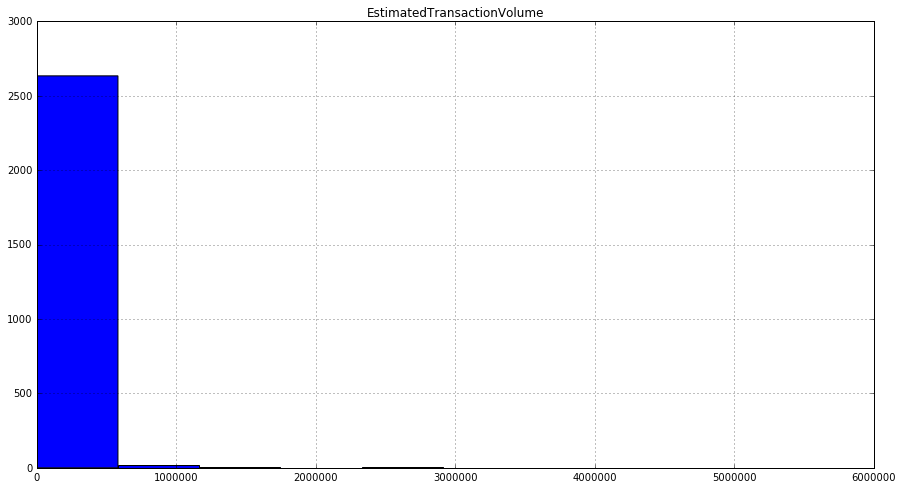
\includegraphics[width=1\linewidth]
    {gfx/estimated-transaction-volume-histogram}}
  \caption{Estimated Transaction Volume Histogram}
  \label{fig:estimated-transaction-volume-histogram}
\end{figure}

\begin{figure}[bth]
  \myfloatalign
  {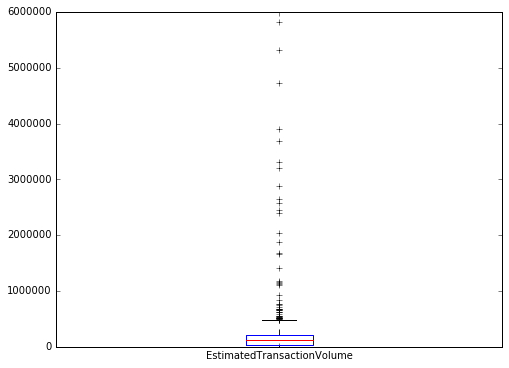
\includegraphics[width=1\linewidth]
    {gfx/estimated-transaction-volume-boxplot}}
  \caption{Estimated Transaction Volume Boxplot}
  \label{fig:estimated-transaction-volume-boxplot}
\end{figure}

\clearpage
%----------------------------------------------------------------------

\subsection{Estimated Transaction Volume USD}
\label{sec:estimated-transaction-volume-usd}

\begin{figure}[bth]
  \myfloatalign
  {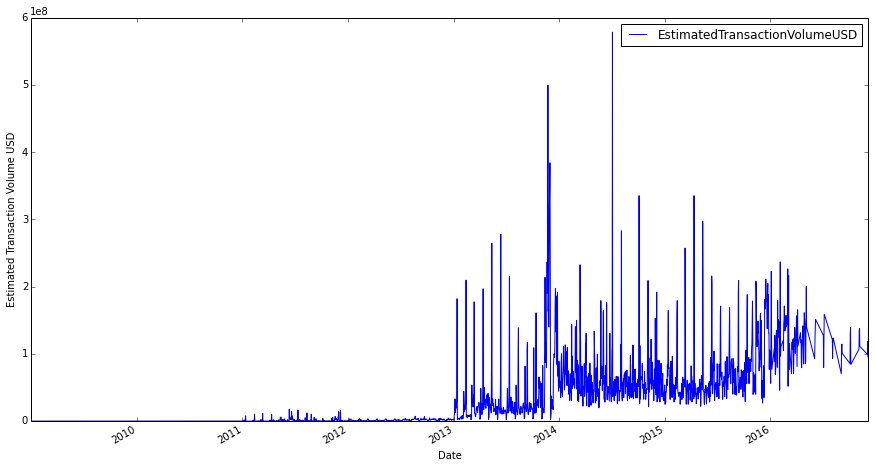
\includegraphics[width=1\linewidth]
    {gfx/estimated-transaction-volume-usd-over-time}}
  \caption{Estimated Transaction Volume USD Over Time}
  \label{fig:estimated-transaction-volume-usd-over-time}
\end{figure}

The Estimated Transaction Volume in USD value, shown in
\autoref{fig:estimated-transaction-volume-usd-over-time}, can be
explained by the average value of Bitcoin, shown in
\autoref{fig:market-price-over-time}, because nearly all the events
are paired in the two figures. There is a small increase in estimated
transaction volume in USD in mid 2011 at the same time than the
average price of Bitcoin increases. Later on, in 2013 there is a
bigger increase in estimated volume that is also reflected in the
average price. Then we have the two biggest peaks around January of
2014 coinciding with the higher average value of Bitcoin (also
represented in two peaks). After that there is decrease in average
price and estimated volume till 2016 where Bitcoin average price
starts to increase at the same time that the estimate transaction
volume increases.

This data-set comprises one integer data point each day, at 18:15:05,
spanning from 03/01/2009 to 03/05/2016.

\begin{table}
  \myfloatalign
  %\small
  \begin{tabularx}{\textwidth}{XX} 
    \toprule
    \tableheadline{Measure} & \tableheadline{Value} \\
    \midrule 
    count  & $2.679e+03$ \\
    median & $2481424.0$ \\
    mean   & $3.018e+07$ \\
    std    & $4.923e+07$ \\
    min    & $0$         \\
    $25$\% & $5.086e+03$ \\
    $50$\% & $2.481e+06$ \\
    $75$\% & $4.761e+07$ \\
    max    & $5.787e+08$ \\
    \bottomrule
  \end{tabularx}
  \caption{Statistical values for \textit{Estimated Transaction Volume USD}}
  \label{tab:estimated-transaction-volume-usd}
\end{table}

\begin{figure}[bth]
  \myfloatalign
  {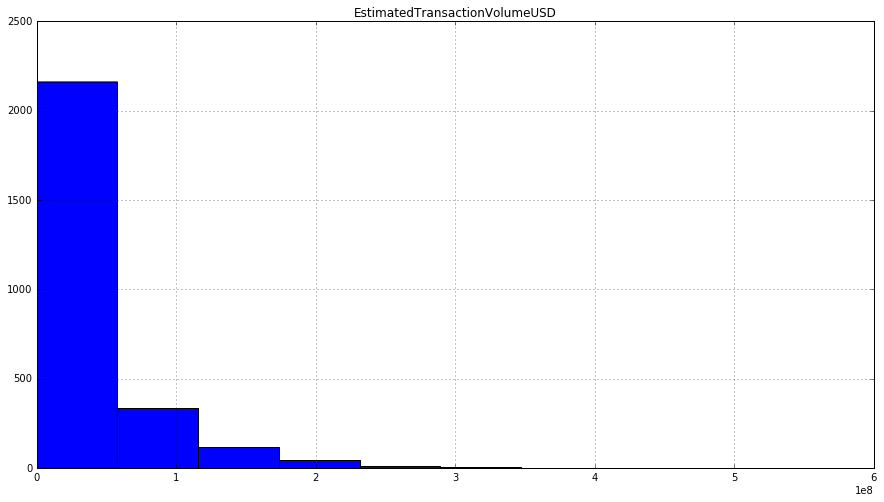
\includegraphics[width=1\linewidth]
    {gfx/estimated-transaction-volume-usd-histogram}}
  \caption{Estimated Transaction Volume USD Histogram}
  \label{fig:estimated-transaction-volume-usd-histogram}
\end{figure}

\begin{figure}[bth]
  \myfloatalign
  {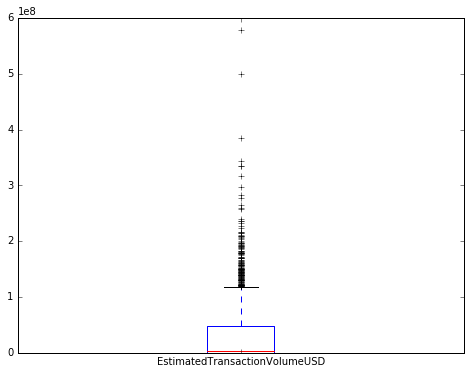
\includegraphics[width=1\linewidth]
    {gfx/estimated-transaction-volume-usd-boxplot}}
  \caption{Estimated Transaction Volume USD Boxplot}
  \label{fig:estimated-transaction-volume-usd-boxplot}
\end{figure}

\clearpage

%----------------------------------------------------------------------

\subsection{Euro price in USD}
\label{sec:euro-price-in-usd}

\begin{figure}[bth]
  \myfloatalign
  {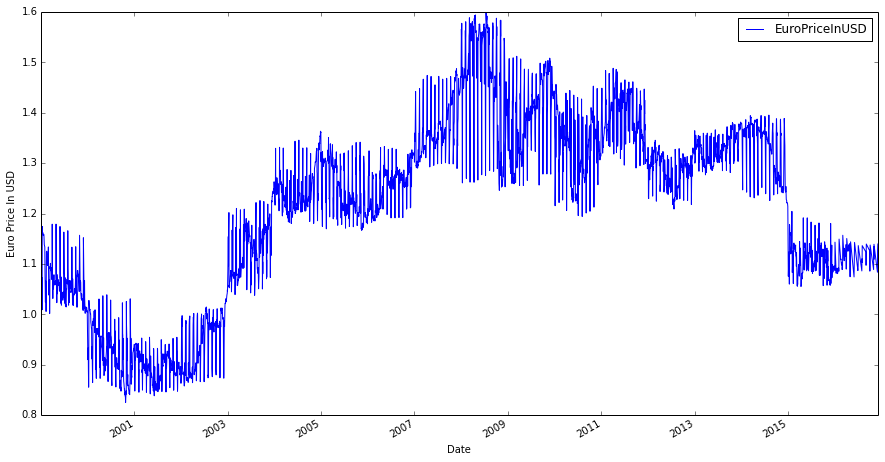
\includegraphics[width=1\linewidth]
    {gfx/euro-price-in-usd-over-time}} 
  \caption{Euro price in USD Over Time}
  \label{fig:euro-price-in-usd-over-time}
\end{figure}

Euro price in USD provided by the European Central Bank from the
creation of the Euro. One real data entry per day, spanning from
04/01/1999 to 10/05/2016.

This dataset has latent values. We have used interpolation in order to
fill the missing values.

As shown in \autoref{fig:euro-price-in-usd-over-time} the value of Euro
has been above that of the USD from its creation, been the period of
2000 through 2003 its closer price to each other. From 2003 to 2007
the price of the Euro increased, coinciding with an increase on the
interest imposed by the BCE. This increase in the interest of the
credits is followed by the collapse of the housing bubble in 2007,
where the price of the Euro kept increasing, altough the interest was
maintained by the BCE until 2009 where the BCE started to lower it.
The increase in the Euro price is probably due to strategies of the
Federal Reserve to lower the price of the USD. Finally in 2015, the
BCE lowered the interests of credits approaching the $0.0\%$, and
that's reflected with a decrease in the price of the Euro with respect
to USD.

\begin{table}
  \myfloatalign
  %\small
  \begin{tabularx}{\textwidth}{XX} 
    \toprule
    \tableheadline{Measure} & \tableheadline{Value} \\
    \midrule 
    count  & $4443$  \\
    mean   & $1.216$ \\
    median & $1.257$ \\
    std    & $0.177$ \\
    min    & $0.825$ \\
    $25$\% & $1.088$ \\
    $50$\% & $1.257$ \\
    $75$\% & $1.345$ \\
    max    & $1.599$ \\
    \bottomrule
  \end{tabularx}
  \caption{Statistical values for \textit{Euro price in USD}}
  \label{tab:euro-price-in-usd}
\end{table}

There are 62 missing values in the data which has been interpolated
after obtaining the descriptive variables of
\autoref{tab:euro-price-in-usd}

\begin{figure}[bth]
  \myfloatalign
  {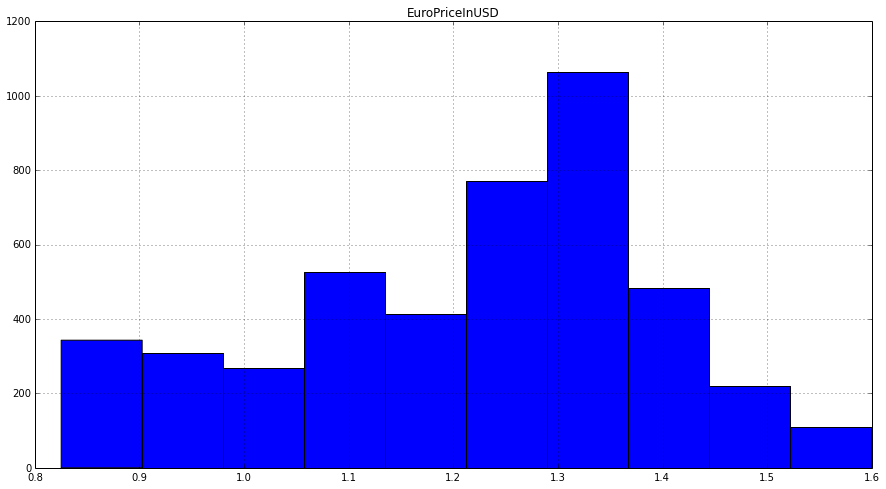
\includegraphics[width=1\linewidth]
    {gfx/euro-price-in-usd-histogram}} 
  \caption{Euro price in USD Histogram}
  \label{fig:euro-price-in-usd-histogram}
\end{figure}

\begin{figure}[bth]
  \myfloatalign
  {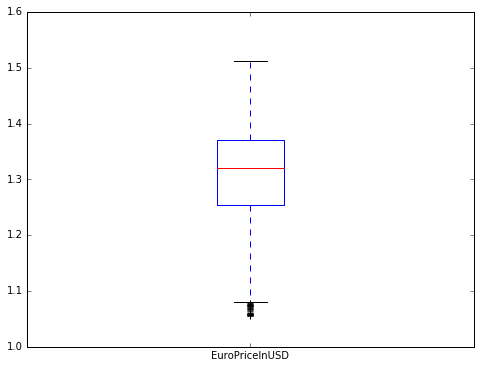
\includegraphics[width=1\linewidth]
    {gfx/euro-price-in-usd-boxplot}}
  \caption{Euro price in USD Boxplot}
  \label{fig:euro-price-in-usd-boxplot}
\end{figure}

\clearpage

%----------------------------------------------------------------------

\subsection{Hash Rate}
\label{sec:hash-rate}

\begin{figure}[bth]
  \myfloatalign
  {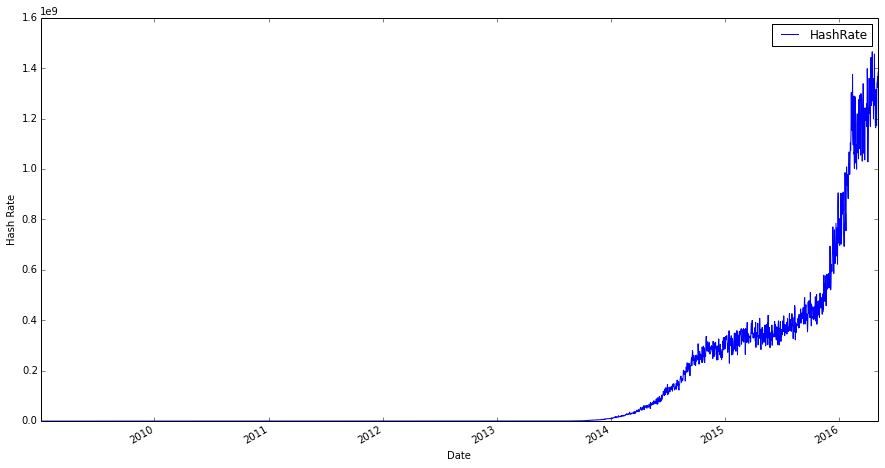
\includegraphics[width=1\linewidth]
    {gfx/hash-rate-over-time}}
  \caption{Hash Rate Over Time}
  \label{fig:hash-rate-over-time}
\end{figure}

The estimated number of giga hashes per second (billions of hashes per
second) the Bitcoin network is performing. The chart in
\autoref{fig:hash-rate-over-time} shows us how mining really started
when Bitcoin raised to its highest value around 2014, reaching more
than 1000\$ per BTC. From that point on, the processing to mining has
increased at approximately $0.2 \times 10^9$ hashes per second, and in
2016, at the same time that the Bitcoin price is starting to increase,
the hash rate started to grow at $1 \times 10^9$ hashes per second in
just a few months. 

This data-set comprises one real number data point each day, at
18:15:05, spanning from 03/01/2009 to 03/05/2016.

\begin{table}
  \myfloatalign
  %\small
  \begin{tabularx}{\textwidth}{XX}
    \toprule
    \tableheadline{Measure} & \tableheadline{Value} \\
    \midrule
    count  & $2.678e+03$ \\
    mean   & $1.265e+08$ \\
    median & $19063.086$ \\
    std    & $2.683e+08$ \\
    min    & $0$         \\
    $25$\% & $2.973e+01$ \\
    $50$\% & $1.906e+04$ \\
    $75$\% & $1.250e+08$ \\
    max    & $1.465e+09$ \\
    \bottomrule
  \end{tabularx}
  \caption{Statistical values for \textit{Hash Rate}}
  \label{tab:hash-rate}
\end{table}

\begin{figure}[bth]
  \myfloatalign
  {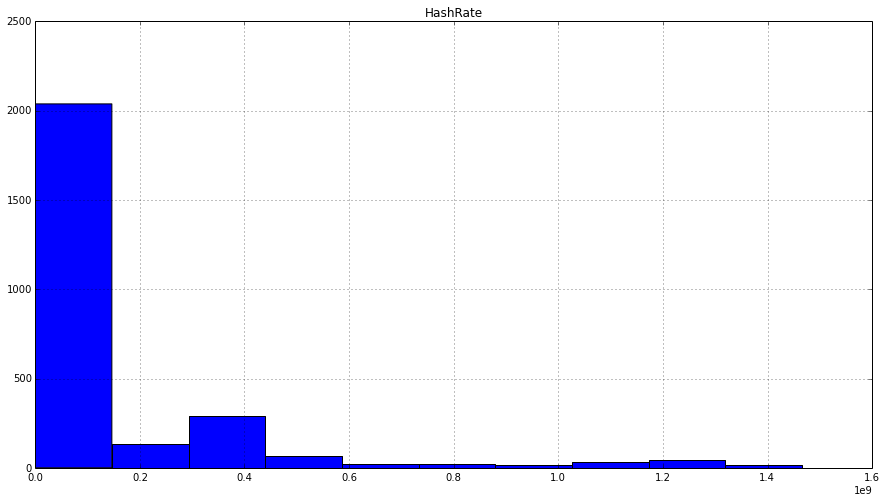
\includegraphics[width=1\linewidth]
    {gfx/hash-rate-histogram}}
  \caption{Hash Rate Histogram}
  \label{fig:hash-rate-histogram}
\end{figure}

\begin{figure}[bth]
  \myfloatalign
  {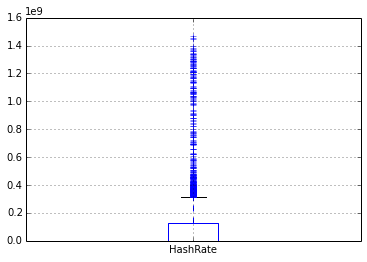
\includegraphics[width=1\linewidth]
    {gfx/hash-rate-boxplot}}
  \caption{Hash Rate Boxplot}
  \label{fig:hash-rate-boxplot}
\end{figure}

\clearpage
%----------------------------------------------------------------------

\subsection{Market Capitalization}
\label{sec:market-cap}

\begin{figure}[bth]
  \myfloatalign
  {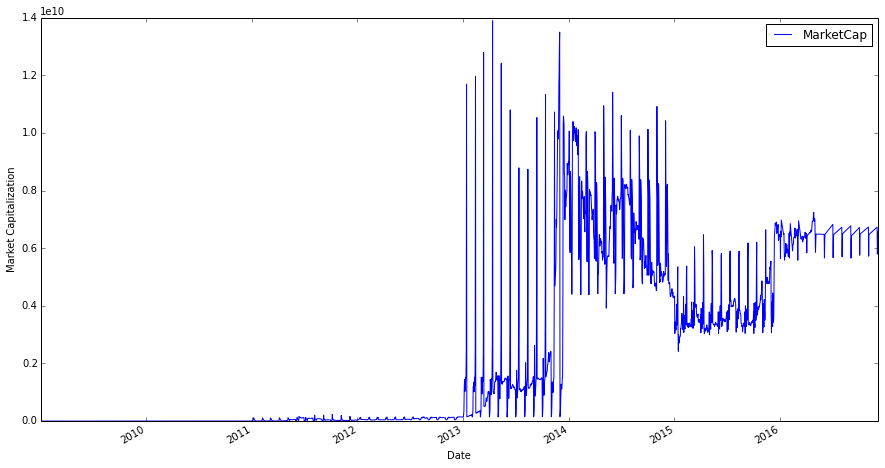
\includegraphics[width=1\linewidth]
    {gfx/market-cap-over-time}}
  \caption{Market Capitalization Over Time}
  \label{fig:market-cap-over-time}
\end{figure}

The total USD value of bitcoin supply in circulation, as calculated by
the daily average market price across major exchanges. This variable
is related to many others, starting with the Bitcoin market price,
with is virtually the same as this one, the number of transactions,
that can explain the fluctuations in the Bitcoin price and different
events. In March 9, 2011, the Bitcoin reaches parity with USD which is
shown in a timid growth in market capitalization followed by a
decrease. After that there isn't a big growth until 2013, where
several things happen, Mega, the cloud storage service, starts
accepting Bitcoins, Internet Archive starts accepting Bitcoins, a new
food service \href{PizzaForCoins.com}{PizzaForCoins.com} accepts
Bitcoins as a payment for food, CoinDesk is launched by Spotify
investor and Coinbase receives 5 million USD in funding. This, and
several other events increase the market capitalization for Bitcoin.

After that there is a decrease in market capitalization of Bitcoin,
maybe because MtGox, the largest exchange operator at the time, was
seized by The United States Department of Homeland Security.

In the second half of 2013, various events happen that can be the
cause of the raise of Bitcoin market capitalization, first, in August
6th, Bitcoin is ruled currency by a Texas judge, then in August 20th,
Bitcoin is ruled as private money in Germany, then in August 28th,
RoboCoin, a Bitcoin ATM manufacturer, starts accepting orders. This
can be the cause of the huge peek at the end of 2013 and start of
2014. There are no clear events in the Bitcoin history that explain
the period after 2014, which leads us to think that the price has been
fluctuating due to trading strategies.

This data-set comprises one real number data point each day, at
18:15:05, spanning from 03/01/2009 to 03/05/2016.

\begin{table}
  \myfloatalign
  %\small
  \begin{tabularx}{\textwidth}{XX} 
    \toprule
    \tableheadline{Measure} & \tableheadline{Value} \\
    \midrule 
    count  & $2.678e+03$     \\
    mean   & $2.072e+09$     \\
    median & $115624066.175$ \\
    std    & $2.879e+09$     \\
    min    & $0$             \\
    $25$\% & $1.005e+06$     \\
    $50$\% & $1.156e+08$     \\
    $75$\% & $3.850e+09$     \\
    max    & $1.390e+10$     \\
    \bottomrule
  \end{tabularx}
  \caption{Statistical values for \textit{Market Capitalization}}
  \label{tab:market-cap}
\end{table}

\begin{figure}[bth]
  \myfloatalign
  {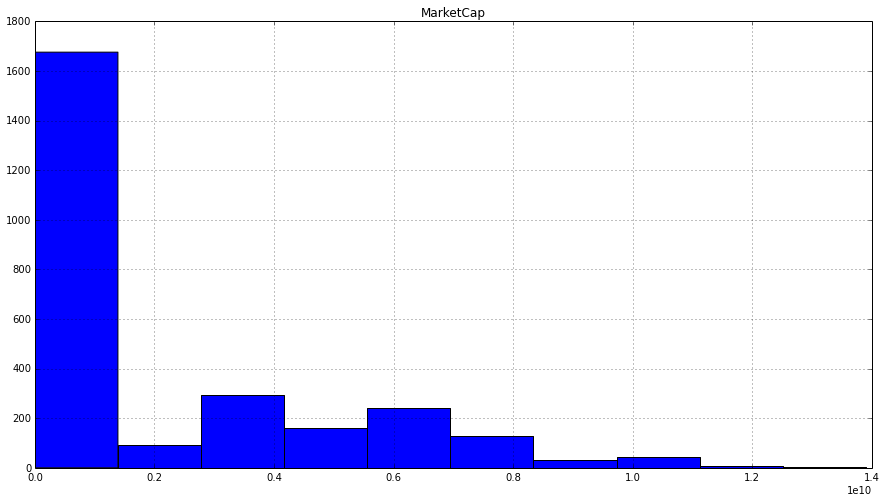
\includegraphics[width=1\linewidth]
    {gfx/market-cap-histogram}}
  \caption{Market Capitalization Histogram}
  \label{fig:market-cap-histogram}
\end{figure}

\begin{figure}[bth]
  \myfloatalign
  {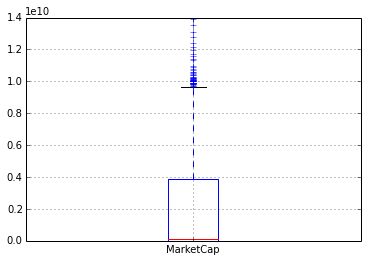
\includegraphics[width=1\linewidth]
    {gfx/market-cap-boxplot}}
  \caption{Market Capitalization Boxplot}
  \label{fig:market-cap-boxplot}
\end{figure}

\clearpage
%----------------------------------------------------------------------

\subsection{Market Price}
\label{sec:market-price}

\begin{figure}[bth]
  \myfloatalign
  {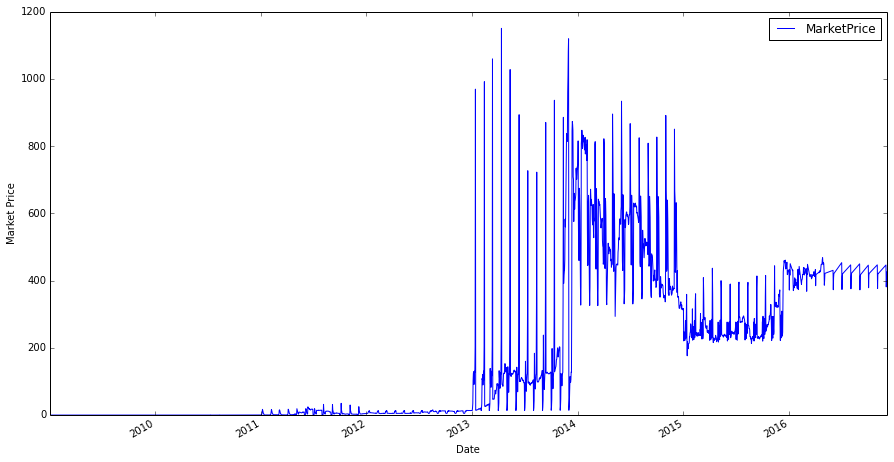
\includegraphics[width=1\linewidth]
    {gfx/market-price-over-time}}
  \caption{Market Price Over Time}
  \label{fig:market-price-over-time}
\end{figure}

Average USD market price across major Bitcoin exchanges.
\autoref{fig:market-price-over-time} is identical to the one in
\autoref{fig:market-cap-over-time} except for the scale. The same
events that produced the market capitalization fluctuation apply to
the market price. Added to that, the average market price across mayor
Bitcoin exchange operators is a variable very closely related to the
market capitalization of Bitcoin.

Is important to note how volatile is the Bitcoin average price,
ranging from nearly $0$ USD to $1100$ USD in just a year, and now, in
2016 fluctuating in a range bigger than $10$ USD on average. This
fluctuations, if predicted, can be very profitable for the trader. 

The data-set comprises one real number data point each day, at
18:15:05, spanning from 03/01/2009 to 03/05/2016.

\begin{table}
  \myfloatalign
  %\small
  \begin{tabularx}{\textwidth}{XX} 
    \toprule
    \tableheadline{Measure} & \tableheadline{Value} \\
    \midrule 
    count  & $2678$    \\
    mean   & $155.924$ \\
    median & $12.378$  \\
    std    & $218.563$ \\
    min    & $0$       \\
    $25$\% & $0.209$   \\
    $50$\% & $12.378$  \\
    $75$\% & $271.335$ \\
    max    & $1151$    \\
    \bottomrule
  \end{tabularx}
  \caption{Statistical values for \textit{Market Price}}
  \label{tab:market-price}
\end{table}

\begin{figure}[bth]
  \myfloatalign
  {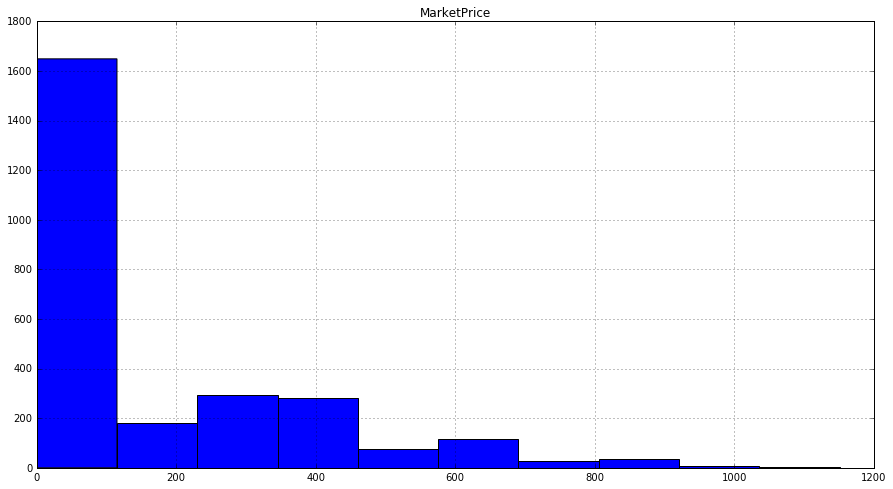
\includegraphics[width=1\linewidth]
    {gfx/market-price-histogram}}
  \caption{Market Price Histogram}
  \label{fig:market-price-histogram}
\end{figure}

\begin{figure}[bth]
  \myfloatalign
  {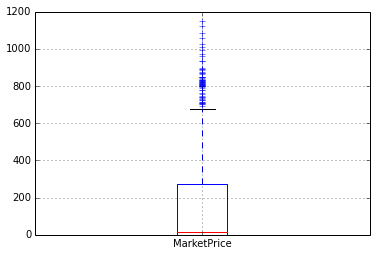
\includegraphics[width=1\linewidth]
    {gfx/market-price-boxplot}}
  \caption{Market Price Boxplot}
  \label{fig:market-price-boxplot}
\end{figure}

\clearpage
%----------------------------------------------------------------------

\subsection{Median Confirmation Time}
\label{sec:median-confirmation-time}

\begin{figure}[bth]
  \myfloatalign
  {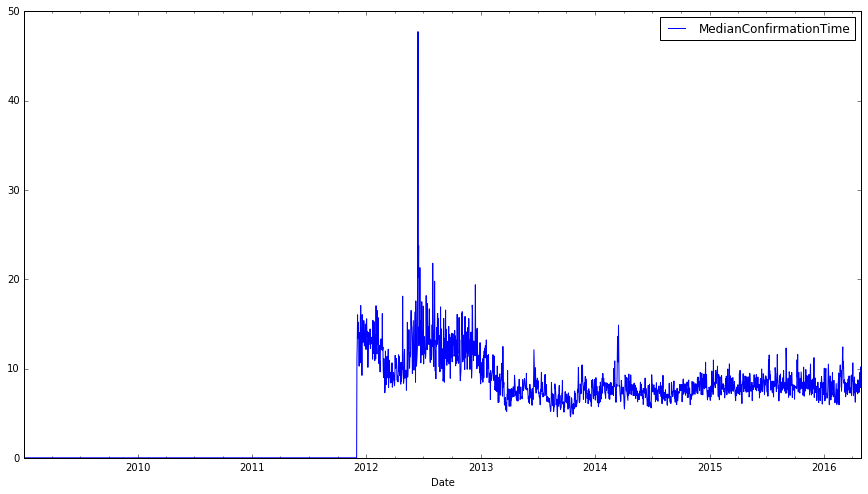
\includegraphics[width=1\linewidth]
    {gfx/median-confirmation-time-over-time}}
  \caption{Median Confirmation Time Over Time}
  \label{fig:median-confirmation-time-over-time}
\end{figure}

The median time for a transaction to be accepted into a mined block
and added to the public ledger (note: only includes transactions with
miner fees). Until the end of 2011, the confirmation time is
negligible. There is an important event that can be related to the
growth of the median confirmation time, and that is the largest
Bitcoin fee in a single transaction, in December 12, 171 Bitcoins was
paids as fee in block 157235.

If we look at \autoref{fig:median-confirmation-time-over-time} there
is a peak in mid 2012, that can coincide with the increase in number
of transactions seen in
\autoref{fig:n-transactions-multiple-over-time}. After that even
though the number of transactions is growing, there is also in
increment in the hash rate, so the number of transactions can be
included in blocks thanks to the amount of miners and their processing
power.

 One real number data point each day, at 18:15:05,
spanning from 03/01/2009 to 03/05/2016.

\begin{table}
  \myfloatalign
  %\small
  \begin{tabularx}{\textwidth}{XX} 
    \toprule
    \tableheadline{Measure} & \tableheadline{Value} \\
    \midrule 
    count  & $2678$   \\
    mean   & $5.385$  \\
    median & $6.975$  \\
    std    & $4.859$  \\
    min    & $0$      \\
    $25$\% & $0$      \\
    $50$\% & $6.975$  \\
    $75$\% & $8.5$    \\
    max    & $47.733$ \\
    \bottomrule
  \end{tabularx}
  \caption{Statistical values for 
    \textit{Median Confirmation Time}}
  \label{tab:median-confirmation-time}
\end{table}

\begin{figure}[bth]
  \myfloatalign
  {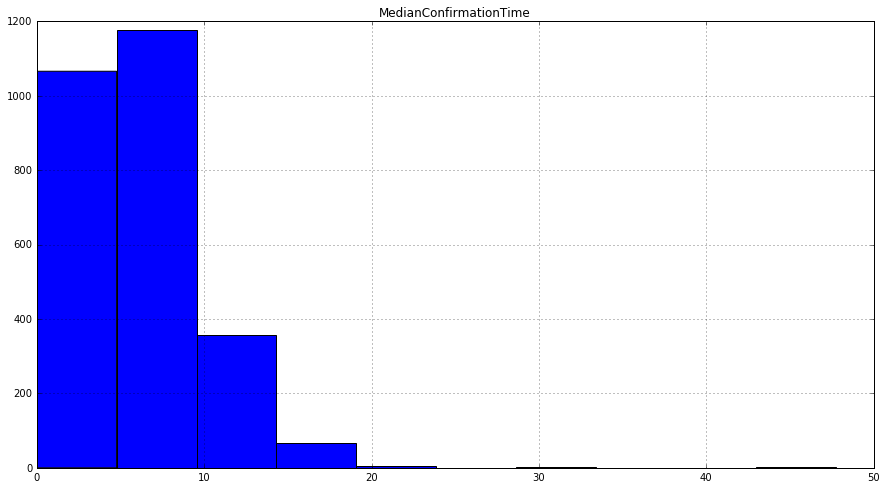
\includegraphics[width=1\linewidth]
    {gfx/median-confirmation-time-histogram}}
  \caption{Median Confirmation Time Histogram}
  \label{fig:median-confirmation-time-histogram}
\end{figure}

\begin{figure}[bth]
  \myfloatalign
  {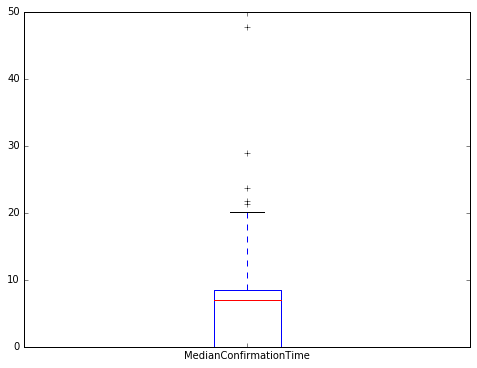
\includegraphics[width=1\linewidth]
    {gfx/median-confirmation-time-boxplot}}
  \caption{Median Confirmation Time Boxplot}
  \label{fig:median-confirmation-time-boxplot}
\end{figure}

\clearpage
%----------------------------------------------------------------------

\subsection{Miners Revenue}
\label{sec:miners-revenue}

\begin{figure}[bth]
  \myfloatalign
  {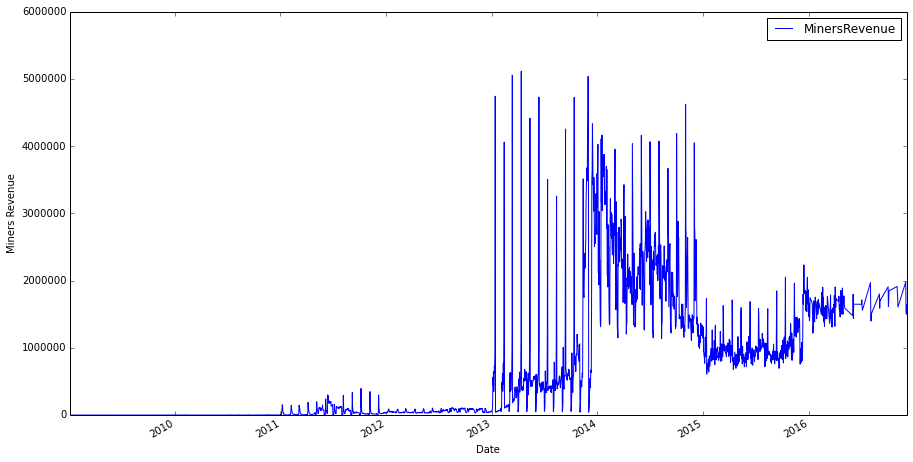
\includegraphics[width=1\linewidth]
    {gfx/miners-revenue-over-time}}
  \caption{Miners Revenue Over Time}
  \label{fig:miners-revenue-over-time}
\end{figure}

Total value of coinbase block rewards and transaction fees paid to
miners, expressed in USD. To understand the rewards and fees, we
include this quote, extracted the 1st of June of 2016 from
\href{https://en.bitcoin.it/wiki/Mining}{Bitcoin.it}:

\textit{``When a block is discovered, the discoverer may award
  themselves a certain number of bitcoins, which is agreed-upon by
  everyone in the network. Currently this bounty is 25 bitcoins; this
  value will halve every 210,000 blocks. [...]. } 

\textit{Additionally, the miner is awarded the fees paid by users
  sending transactions. The fee is an incentive for the miner to
  include the transaction in their block. In the future, as the number
  of new bitcoins miners are allowed to create in each block dwindles,
  the fees will make up a much more important percentage of mining
  income.''}

Taking the previous quote into consideration, we know that the miner
reward is fixed, so its fluctuation will depend upon the price of the
Bitcoin itself, therefore the resemblance between miners revenue
(\autoref{fig:miners-revenue-over-time}) and Bitcoin price
(\autoref{fig:market-price-over-time}).

In 2016, the transaction fees represent a very small amount of the
BTCs of the miners revenue. We can see in
\autoref{tab:cost-per-transaction} that the average transaction has a
value of $9.727$. On the other hand, the average number of
transactions per block $306.632$. Thus the expected revenue due to
fees of a single miner is $9.727 \times 306.632 = $
$2982.731$ USD.

If we analyze the revenue thanks to the reward of discovering a block
we have that the average market price of the
Bitcoin(\autoref{tab:market-price}) is $155.924$
USD and the reward is $25$
BTC per block discovered, that makes an amount of
$155.924 \times 25 = 3898.109$
USD per block discovered. Added to that, we have to keep in mind that,
as of June the 2nd, the current price of Bitcoin is $536.99$
USD, which makes the rewards value increase to
$536.99 \times 25 = 13424.75$
USD per blocked discovered. We can conclude that nowadays, the main
source of revenues for miners is the block discovery, but in the
future, as it goes getting harder to discover blocks, the fees will
start to be an important source of income for miners.

This data-set comprises one real number data point each day, at
18:15:05, spanning from 03/01/2009 to 03/05/2016.

\begin{table}
  \myfloatalign
  %\small
  \begin{tabularx}{\textwidth}{XX} 
    \toprule
    \tableheadline{Measure} & \tableheadline{Value} \\
    \midrule 
    count  & $2678$        \\
    mean   & $638331.424$  \\
    median & $85611.647$   \\
    std    & $911565.967$  \\
    min    & $0.000$       \\
    $25$\% & $1895.375$    \\
    $50$\% & $85611.647$   \\
    $75$\% & $1023087.365$ \\
    max    & $5117346$     \\
    \bottomrule
  \end{tabularx}
  \caption{Statistical values for \textit{Miners Revenue}}
  \label{tab:miners-revenue}
\end{table}

\begin{figure}[bth]
  \myfloatalign
  {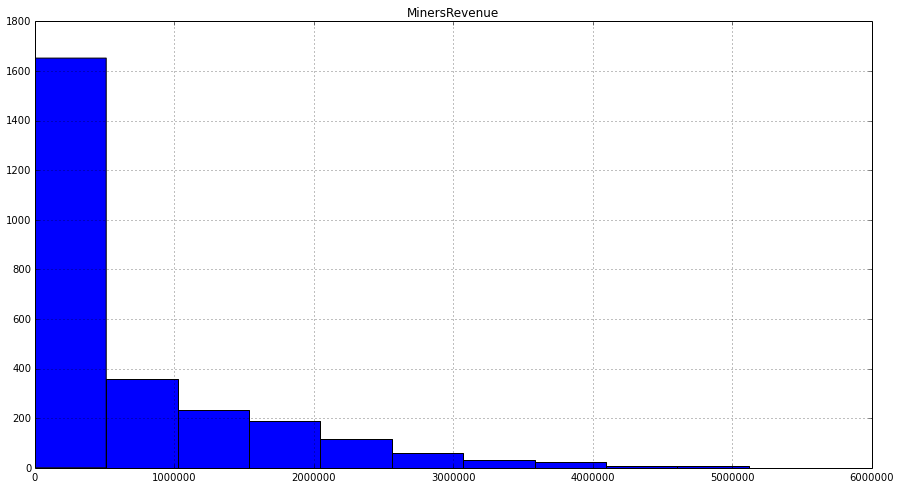
\includegraphics[width=1\linewidth]
    {gfx/miners-revenue-histogram}}
  \caption{Miners Revenue Histogram}
  \label{fig:miners-revenue-histogram}
\end{figure}

\begin{figure}[bth]
  \myfloatalign
  {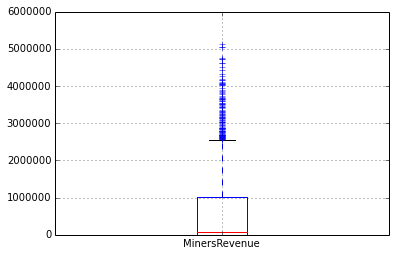
\includegraphics[width=1\linewidth]
    {gfx/miners-revenue-boxplot}}
  \caption{Miners Revenue Boxplot}
  \label{fig:miners-revenue-boxplot}
\end{figure}

\clearpage
%----------------------------------------------------------------------

\subsection{Network Deficit}
\label{sec:network-deficit}

\begin{figure}[bth]
  \myfloatalign
  {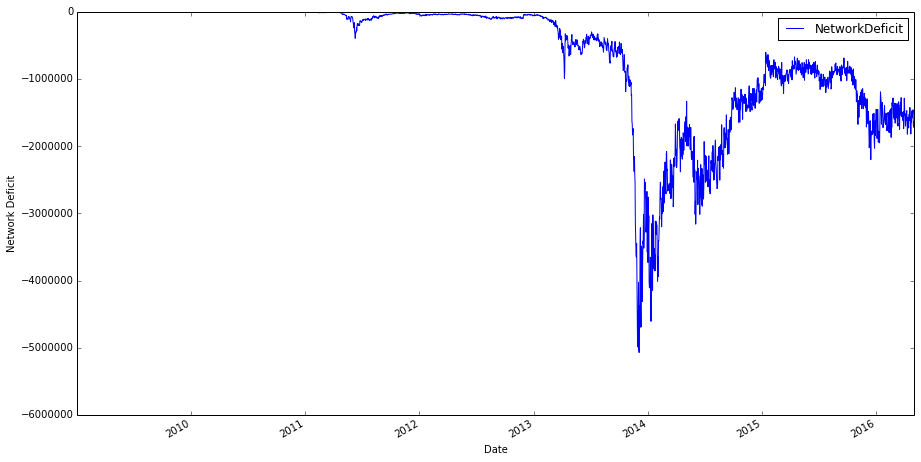
\includegraphics[width=1\linewidth]
    {gfx/network-deficit-over-time}}
  \caption{Network Deficit Over Time}
  \label{fig:network-deficit-over-time}
\end{figure}

Shows difference between transaction fees and cost of Bitcoin mining
in USD. This definition, given by
\href{https://blockchain.info/charts}{BlockChain.info} can be a little
bit misleading, because it's not clear what the \textit{cost of
  Bitcoin mining} means. After some research, we found in
\href{http://bitcoin.stackexchange.com/questions/10230/how-is-network-deficit-calculated}{StackExchange}
that the cost of Bitcoin mining is the reward from Bitcoin mining. So
the network deficit, is the difference between transaction fees and
reward for mining. There is a lot of discussion about what this
variable represents, and how to interpret it. For example:

``\textit{So at the current rate of 1 tps, the average transaction fee
  would need to rise to \$5 worth of BTC to keep mining at its current
  economic strength. This would drastically reduce write access to
  Bitcoin, and might not even be achievable due to consumer choice
  (growing preference among potential adoptees for market alternatives
  like traditional finance, alt-blockchains, etc as the average tx fee
  increases).}

\textit{While decentralization has been the main focus of the block
  size debate, hashrate (mining revenues) and accessibility (cost of
  transaction) are also important metrics of network utility and
  health, and should be taken into consideration.}

\textit{The lower the maximum transaction throughput, the more
  expensive transactions need to be to maintain current mining
  revenues. The optimal block size limit will strike the right balance
  between mining decentralization, miner revenue, and write
  accessibility, and not exclude any of these factors in its focus.}''

What we see in \autoref{fig:network-deficit-over-time} is that as
mentioned before in \autoref{sec:miners-revenue}, the revenues of
miners are mostly due to the rewards of block discovery instead of the
fees produced in transactions. This can be interpreted as a network
inmaturity, because miners, which are the main supporters of the
Bitcoin network, rely mostly on the Bitcoin inflation to make profit,
instead of the transactions and associated fees.

It's easy to see the relationship between the network deficit and the
Bitcoin market price by noticing that
\autoref{fig:network-deficit-over-time} and
\autoref{fig:market-price-over-time} are nearly simetrical in the X
axis. So, the higher the price of bitcoin, the higher is the deficit
(though is represented in negative numbers).

This data-set comprises one real number data point each day, at
18:15:05, spanning from 03/01/2009 to 03/05/2016.


\begin{table}
  \myfloatalign
  %\small
  \begin{tabularx}{\textwidth}{XX} 
    \toprule
    \tableheadline{Measure} & \tableheadline{Value} \\
    \midrule 
    count  & $2678$         \\
    mean   & -$631395.059$  \\
    median & -$84958.600$   \\
    std    & $903713.147$   \\
    min    & -$5068845.988$ \\
    $25$\% & -$1009464.098$ \\
    $50$\% & -$84958.600$   \\
    $75$\% & -$1895.354$    \\
    max    & $0$            \\
    \bottomrule
  \end{tabularx}
  \caption{Statistical values for \textit{Network Deficit}}
  \label{tab:network-deficit}
\end{table}

\begin{figure}[bth]
  \myfloatalign
  {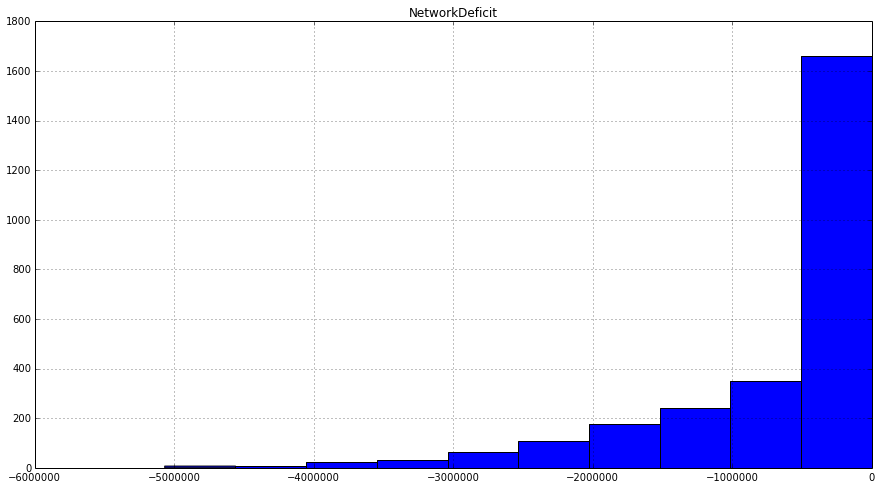
\includegraphics[width=1\linewidth]
    {gfx/network-deficit-histogram}}
  \caption{Network Deficit Histogram}
  \label{fig:network-deficit-histogram}
\end{figure}

\begin{figure}[bth]
  \myfloatalign
  {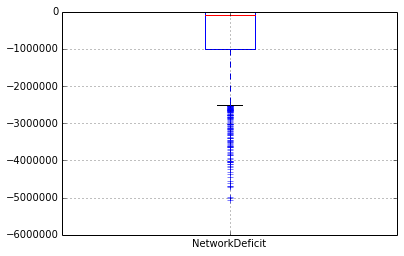
\includegraphics[width=1\linewidth]
    {gfx/network-deficit-boxplot}}
  \caption{Network Deficit Boxplot}
  \label{fig:network-deficit-boxplot}
\end{figure}

\clearpage
%----------------------------------------------------------------------

\subsection{Number of Transactions}
\label{sec:n-transactions-multiple}

\begin{figure}[bth]
  \myfloatalign
  {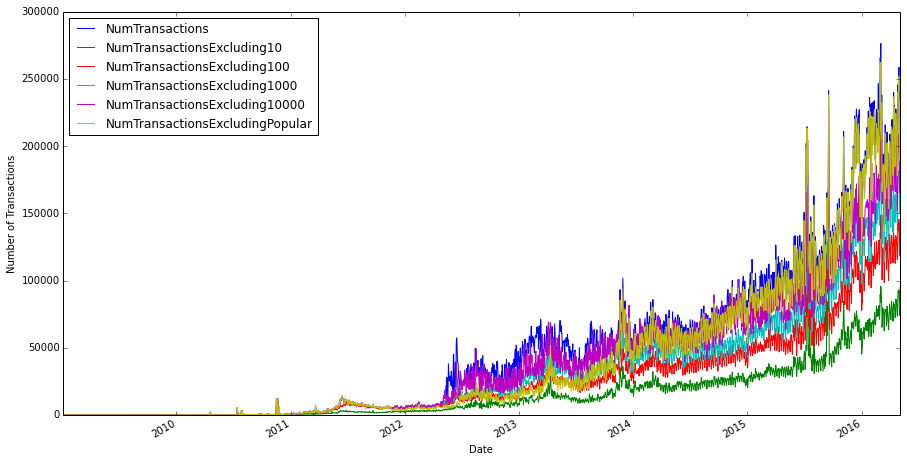
\includegraphics[width=1\linewidth]
    {gfx/n-transactions-multiple-over-time}}
  \caption{Number of Transactions Over Time}
  \label{fig:n-transactions-multiple-over-time}
\end{figure}

Here we analyze a compound set of variables: number of transactions,
number of transactions excluding chains longer than 10, 100, 1000 and
10000, and number of transactions excluding the 100 most popular
addresses. 

The number of transactions is defined as ``\textit{The number of daily
  confirmed Bitcoin transactions}''. As for long chains, we include a
quote from
\href{http://www.ofnumbers.com/2015/01/22/slicing-data-what-comprises-blockchain-transactions/}{Tim
  Swanson} that explains the origin of the term and why can be useful:
``\textit{questions have arisen over a series of what some call “long
  chains.” Last month several commentators on a popular thread on
  Hacker News identified thousands of small transactions originating
  from a single source. The source was continually sending
  transactions and paid transaction fees for each of them. The reason
  this struck many as odd as a rational actor would simply bundle the
  transactions together to save on transaction fees.}

\textit{ While there are likely different motivations for doing so,
  one reason for why this was occurring was that the originating
  source was attempting to delink or otherwise mix and tumble coins to
  make it difficult to “dox” or identify the originating source. But
  it could also be a faucet and at one point even pools paid out
  miners using chained transactions, perhaps some still do.}''


The number of transactions represented in blue color in
\autoref{fig:n-transactions-multiple-over-time} show a moderated
growth compared to that of the market price or market capitalization.
That may be because this variable doesn't depend on the inflation of
the Bitcoin, and there aren't exagerated fluctuation. We see that even
the price of the Bitcoin is not at its peak in 2016, the number of
transactions are in the higher point so far in the Bitcoin history.
It's also possible to see the relatioship between the different curves
excluding ``long chains'', where as the ``long chains'' are removed
the number of transactions decrease, although the tendency is similar.

Regarding \textit{number of transactions excluding popular}, is useful
to show whether there is a dependecy of a small number of actors in
the Bitcoin network. What we see in
\autoref{fig:n-transactions-multiple-over-time} is that,
\textit{number of transactions excluding popular} in yellow, is
growing independent from the 100 most popular addresses. While until
2014 this addresses added a substantial amount of transactions to the
overall count, from that point on, the count between the total
transactions and \textit{number of transactions excluding popular} is
similar.

This data-set comprises six integer data point each day, at 18:15:05,
spanning from 03/01/2009 to 03/05/2016.

\begin{table}
  \myfloatalign
  \tiny
  \begin{tabularx}{\textwidth}{XXXXXXX} 
    \toprule
    \tableheadline{Measure} &
    \tableheadline{NumTransactions} &
    \tableheadline{Ex-10} &
    \tableheadline{Ex-100} &
    \tableheadline{Ex-1000} &
    \tableheadline{Ex-10000} &
    \tableheadline{Ex-Popular} \\
    \midrule                                                                                     
    count  & $2678$      & $2678$      & $2678$      & $2678$      & $2678$      & $2678$      \\
    mean   & $47255.265$ & $15589.578$ & $26050.881$ & $32665.966$ & $39117.017$ & $40400.536$ \\
    median & $31214$     & $7115$      & $12810$     & $16915$     & $22558$     & $12597.5$   \\
    std    & $56769.848$ & $20367.504$ & $32164.862$ & $40035.066$ & $46391.775$ & $55357.260$ \\
    min    & $0$         & $0$         & $0$         & $0$         & $0$         & $0$         \\
    $25$\  & $501.5$     & $337$       & $426.25$    & $486.25$    & $501.5$     & $501.5$     \\
    $50$\  & $31214$     & $7115$      & $12810$     & $16915$     & $22558$     & $12597.5$   \\
    $75$\  & $69853$     & $23695.5$   & $39936.75$  & $50210.75$  & $61130$     & $63434.25$  \\
    max    & $276448$    & $157002$    & $187035$    & $206184$    & $227830$    & $262461$    \\
    \bottomrule
  \end{tabularx}
  \caption{Statistical values for \textit{Number of Transactions}}
  \label{tab:n-transactions-multiple}
\end{table}

\begin{figure}[bth]
  \myfloatalign
  {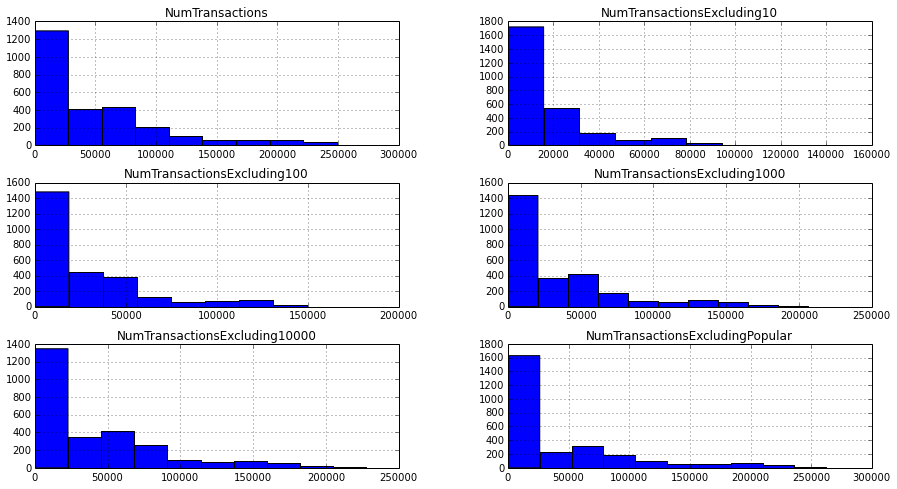
\includegraphics[width=1\linewidth]
    {gfx/n-transactions-multiple-histogram}}
  \caption{Number of Transactions Histogram}
  \label{fig:n-transactions-multiple-histogram}
\end{figure}

\begin{figure}[bth]
  \myfloatalign
  {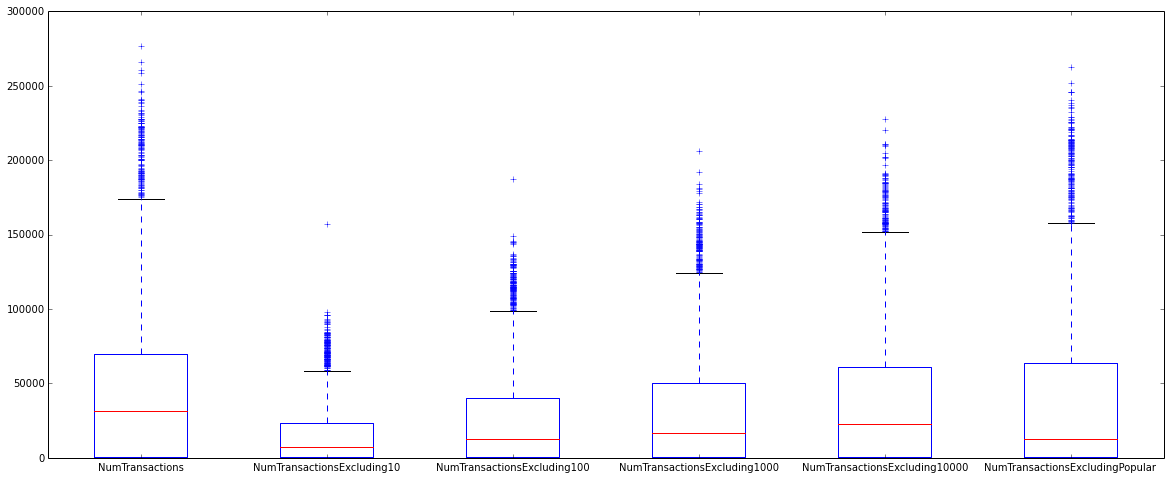
\includegraphics[width=1\linewidth]
    {gfx/n-transactions-multiple-boxplot}}
  \caption{Number of Transactions Boxplot}
  \label{fig:n-transactions-multiple-boxplot}
\end{figure}

\clearpage
%----------------------------------------------------------------------

\subsection{Number of Transactions Per Block}
\label{sec:n-transactions-per-block}

\begin{figure}[bth]
  \myfloatalign
  {\includegraphics[width=1\linewidth]
    {gfx/n-transactions-per-block-over-time}}
  \caption{Number of Transactions Per Block
    Over Time}
  \label{fig:n-transactions-per-block-over-time}
\end{figure}

This variable represents the average number of transactions per block.
The way transactions are added to the Bitcoin network is by adding
them to a block. This operation is done by miners, that receive a fee
(that can be zero) to do this operation. As mentioned before, today,
miners revenue are due mostly to the discovery of new blocks instead
of fees, nonetheless fees is another source of income. A miner can
choose not to include transactions in the mined blocks, and that would
go against the healthy growth of the Bitcoin network. Fortunately,
\autoref{fig:n-transactions-per-block-over-time} shows that the amount
of transactions per block is increasing, this way Bitcoin networks can
keep growing relying in miners to process transactions. On top of
that, the average amount of transactions per block since mid 2015 is
greater than $1000$, given that the average cost per transaction is
$9.727$ which gives an average revenue of $9727.391$ USD per block
for miner for this period.

This data-set comprises one integer data point each day, at 18:15:05,
spanning from 03/01/2009 to 28/04/2016.

\begin{table}
  \myfloatalign
  %\small
  \begin{tabularx}{\textwidth}{XX} 
    \toprule
    \tableheadline{Measure} & \tableheadline{Value} \\
    \midrule 
    count  & $2673$    \\
    mean   & $306.632$ \\
    median & $205$     \\
    std    & $377.986$ \\
    min    & $1$       \\
    $25$\% & $2$       \\
    $50$\% & $205$     \\
    $75$\% & $435$     \\
    max    & $2036$    \\
    \bottomrule
  \end{tabularx}
  \caption{Statistical values for \textit{Number of Transactions 
      Per Block}}
  \label{tab:n-transactions-per-block}
\end{table}

\begin{figure}[bth]
  \myfloatalign
  {\includegraphics[width=1\linewidth]
    {gfx/n-transactions-per-block-histogram}}
  \caption{Number of Transactions Per Block
    Histogram}
  \label{fig:n-transactions-per-block-histogram}
\end{figure}

\begin{figure}[bth]
  \myfloatalign
  {\includegraphics[width=1\linewidth]
    {gfx/n-transactions-per-block-boxplot}}
  \caption{Number of Transactions Per Block
    Boxplot}
  \label{fig:n-transactions-per-block-boxplot}
\end{figure}

\clearpage
%---------------------------------------------------------------------- 

\subsection{Number of Total Transactions}
\label{sec:n-transactions-total}

\begin{figure}[bth]
  \myfloatalign
  {\includegraphics[width=1\linewidth]
    {gfx/n-transactions-total-over-time}}
  \caption{Number of Total Transactions
    Over Time}
  \label{fig:n-transactions-total-over-time}
\end{figure}


Total number of transactions data in
\autoref{fig:n-transactions-total-over-time} show that the growth is
exponential. It can be seen in
\autoref{fig:n-transactions-multiple-over-time} that the number of
transactions per day is increasing, from that we can assume that the
growth of accumulated number of transactions over time is going to
increase in a nearly exponential way.

This data-set comprises one integer data point each day, at 18:15:05,
spanning from 03/01/2009 to 03/05/2016.

\begin{table}
  \myfloatalign
  %\small
  \begin{tabularx}{\textwidth}{XX} 
    \toprule
    \tableheadline{Measure} & \tableheadline{Value} \\
    \midrule 
    count  & $2.678e+03$ \\
    mean   & $2.491e+07$ \\
    median & $6685067$   \\
    std    & $3.308e+07$ \\
    min    & $1$         \\
    $25$\% & $1.384e+05$ \\
    $50$\% & $6.685e+06$ \\
    $75$\% & $4.191e+07$ \\
    max    & $1.265e+08$ \\
    \bottomrule
  \end{tabularx}
  \caption{Statistical values for \textit{Number of Total
      Transactions}}
  \label{tab:n-transactions-total}
\end{table}

\begin{figure}[bth]
  \myfloatalign
  {\includegraphics[width=1\linewidth]
    {gfx/n-transactions-total-histogram}}
  \caption{Number of Total Transactions
    Histogram}
  \label{fig:n-transactions-total-histogram}
\end{figure}

\begin{figure}[bth]
  \myfloatalign
  {\includegraphics[width=1\linewidth]
    {gfx/n-transactions-total-boxplot}}
  \caption{Number of Total Transactions
    Boxplot}
  \label{fig:n-transactions-total-boxplot}
\end{figure}

\clearpage
%---------------------------------------------------------------------- 

\subsection{Number of Unique Addresses}
\label{sec:n-unique-addresses}

\begin{figure}[bth]
  \myfloatalign
  {\includegraphics[width=1\linewidth]
    {gfx/n-unique-addresses-over-time}}
  \caption{Number of Unique Addresses
    Over Time}
  \label{fig:n-unique-addresses-over-time}
\end{figure}

The total number of unique addresses used on the Bitcoin blockchain. A
unique adress, as defined by
\href{https://en.bitcoin.it/wiki/Address}{Bitcoin.it}: ``\textit{A
  Bitcoin address, or simply address, is an identifier of 26-35
  alphanumeric characters, beginning with the number 1 or 3, that
  represents a possible destination for a bitcoin payment.}'' This
variable is closely related to the number of transactions made in the
network. When compared,
\autoref{fig:n-transactions-multiple-over-time} and
\autoref{fig:n-unique-addresses-over-time} show a resemblance not only
in the events that produce the local maximums but also in the growth.

This data-set comprises one integer data point each day, at 18:15:05,
spanning from 03/01/2009 to 03/05/2016.

\begin{table}
  \myfloatalign
  %\small
  \begin{tabularx}{\textwidth}{XX} 
    \toprule
    \tableheadline{Measure} & \tableheadline{Value} \\
    \midrule 
    count  & $2678$       \\
    mean   & $86921.616$  \\
    median & $29205.5$    \\
    std    & $112219.880$ \\
    min    & $0$          \\
    $25$\% & $609.25$     \\
    $50$\% & $29205.5$    \\
    $75$\% & $152308.5$   \\
    max    & $483756$     \\
    \bottomrule
  \end{tabularx}
  \caption{Statistical values for \textit{Number of Unique Addresses}}
  \label{tab:n-unique-addresses}
\end{table}

\begin{figure}[bth]
  \myfloatalign
  {\includegraphics[width=1\linewidth]
    {gfx/n-unique-addresses-histogram}}
  \caption{Number of Unique Addresses
    Histogram}
  \label{fig:n-unique-addresses-histogram}
\end{figure}

\begin{figure}[bth]
  \myfloatalign
  {\includegraphics[width=1\linewidth]
    {gfx/n-unique-addresses-boxplot}}
  \caption{Number of Unique Addresses
    Boxplot}
  \label{fig:n-unique-addresses-boxplot}
\end{figure}

\clearpage
%--------------------------------------------------------------------- 

\subsection{Output Volume}
\label{sec:output-volume}

\begin{figure}[bth]
  \myfloatalign
  {\includegraphics[width=1\linewidth]
    {gfx/output-volume-over-time}}
  \caption{Output Volume
    Over Time}
  \label{fig:output-volume-over-time}
\end{figure}

The total value of all transaction outputs per day (includes coins
returned to the sender as change). It's easier to understand to
meaning of output and change in the bitcoin world with an explanation
given by a user nicknamed \textit{DeathAndTaxes} in
\href{https://bitcointalk.org/index.php?topic=99593.0}{Bitcointalk.org}:

``\textit{Bitcoin can only create transactions by using as the input
  an ENTIRE prior unspent output. The most important thing to realize
  is that Bitcoin tx have inputs and outputs. The "value" of your
  wallet is an abstraction. It is simply your client (software which
  analyzes the wallet) taking a SUM of all the unspent outputs which
  you have private keys for. The input of a tx is the output of a
  PRIOR tx. You can only use unspent outputs in a new tx. Once they
  are part of a tx they can never be used again ("spent").}

\textit{Say you I send you 50 BTC (for simplicity lets assume this is
  compromised of a single 50 BTC output). No matter how you spend that
  the input for the tx will be 50 BTC.}

\textit{Want to spend 20 BTC? Input: 50 BTC Output: 20 BTC + 30 BTC
  "change" back to an address you control. Want to spend 1 BTC? Input:
  50 BTC Output: 1 BTC + 49 BTC "change" back to an address you
  control.}''

Output can be due to three circumstances, large amout of transactions,
transactions of big amount of Bitcoins, and big amount of change
returned to sender. The peak of 2013 is clearly due to change received
by sender as \textit{DeathAndTaxes} explains: ``\textit{In the early
  days of Bitcoin there really was nothing to "spend" it on so most tx
  tended to be accumulation. This resulted in most addresses having
  very large unspent outputs. As people started "breaking" up those
  unspent outputs in tx involving smaller amounts most of the volume
  WAS change.}''

This data-set comprises one real number data point each day, at
18:15:05, spanning from 03/01/2009 to 03/05/2016.

\begin{table}
  \myfloatalign
  %\small
  \begin{tabularx}{\textwidth}{XX} 
    \toprule
    \tableheadline{Measure} & \tableheadline{Value} \\
    \midrule 
    count  & $2679$         \\
    mean   & $1134859.870$  \\
    median & $661019.796$   \\
    std    & $2333431.889$  \\
    min    & $0$            \\
    $25$\% & $73233.013$    \\
    $50$\% & $661019.796$   \\
    $75$\% & $1286432.155$  \\
    max    & $45992222.558$ \\
    \bottomrule
  \end{tabularx}
  \caption{Statistical values for \textit{Output Volume}}
  \label{tab:output-volume}
\end{table}

\begin{figure}[bth]
  \myfloatalign
  {\includegraphics[width=1\linewidth]
    {gfx/output-volume-histogram}}
  \caption{Output Volume
    Histogram}
  \label{fig:output-volume-histogram}
\end{figure}

\begin{figure}[bth]
  \myfloatalign
  {\includegraphics[width=1\linewidth]
    {gfx/output-volume-boxplot}}
  \caption{Output Volume
    Boxplot}
  \label{fig:output-volume-boxplot}
\end{figure}

\clearpage
%--------------------------------------------------------------------- 

\subsection{Standard \& Poors 500}
\label{sec:standard-and-poors-500}

\begin{figure}[bth]
  \myfloatalign
  {\includegraphics[width=1\linewidth]
    {gfx/standard-and-poors-500-over-time}}
  \caption{Standard Output Volume Poors 500
    Over Time}
  \label{fig:standard-and-poors-500-over-time}
\end{figure}

From the
\href{https://en.wikipedia.org/wiki/S\%26P_500_Index}{Wikipedia}:

``\textit{The Standard \& Poor's 500, often abbreviated as the S\&P
  500, or just "the S\&P", is an American stock market index based on
  the market capitalizations of 500 large companies having common
  stock listed on the NYSE or NASDAQ. The S\&P 500 index components
  and their weightings are determined by S\&P Dow Jones Indices. It
  differs from other U.S. stock market indices, such as the Dow Jones
  Industrial Average or the Nasdaq Composite index, because of its
  diverse constituency and weighting methodology. It is one of the
  most commonly followed equity indices, and many consider it one of
  the best representations of the U.S. stock market, and a bellwether
  for the U.S. economy. The National Bureau of Economic Research has
  classified common stocks as a leading indicator of business cycles.}

\textit{[...]}

\textit{On August 12, 1982, the index closed at 102.42.}

\textit{The index reached a relative intraday high—which was not
  exceeded for over seven years—of 1,552.87, on March 24, 2000, during
  the dot-com bubble. The index then declined by approximately 50\%,
  to 768.63, on October 10, 2002, during the stock market downturn of
  2002. On May 30, 2007, the S\&P 500 closed at 1,530.23, to set its
  first all-time closing high in more than seven years. Although the
  index achieved a new all-time intraday high on October 11, 2007, at
  1,576.09, following a record close of 1,565.15 on October 9, the
  index finished 2007 at 1,468.36 points—just below its 1999 annual
  close. Less than a month later, it dropped to 1,400, and would not
  see similar levels again for five years.}

\textit{In mid-2007, the subprime mortgage crisis spread to the wider
  U.S. financial sector. The resulting situation became acute in
  September 2008, ushering in a period of unusual market volatility,
  encompassing record 100-point swings in both directions and reaching
  the highest levels since 1929. On November 20, 2008, the index
  closed at 752.44, its lowest since early 1997. A modest recovery the
  following day still left the index down 45.5\% for the year. This
  year-to-date loss was the greatest since 1931, when the broad market
  declined more than 50\%. The index closed the year at 903.25, for a
  loss of 38.5\%. The market continued to decline in early 2009,
  surrounding the financial crisis of 2008. The index reached a nearly
  13-year low, closing at 676.53, on March 9, 2009.}

\textit{On March 23, 2009, the S\&P 500 marked a 20\% gain when it hit
  822.92. The Dow Jones Industrial Average soon followed. The close
  for 2009 was 1,115.10, making it the second-best year of the decade.
  On April 14, 2010 the index broke 1200 closing at 1210.65, but by
  July 2, 2010 it had closed at 1022.58. On April 29, 2011, the index
  closed at 1363.61, but it had a sharp drop in August and briefly
  broke 1100 in October (with the VIX hitting 40). Gains continued
  despite significant volatility amid electoral and fiscal
  uncertainty, and the 2012 close of the S\&P 500 following QE3 was
  its third-highest ever, at 1,426.22 points. Many people hated the
  bull market. On March 28, 2013, it closed above the closing high
  from 2007. On April 10, 2013, it also closed above the intraday high
  from 2007.}

\textit{On May 3, 2013—more than 13 years since its first close above
  1,500—the S\&P 500 closed above 1,600 for the first time, at
  1,614.42. This would be the first of three 100-point milestones in
  2013: 1,600 on May 3, 2013; 1,700 on August 1, 2013; and 1,800 on
  November 22, 2013. The S\&P 500 closed out 2013 at a record high,
  finishing the December 31, 2013, trading day at 1,848.36. On May 23,
  2014, the index for the first time closed above 1,900, at 1,900.53.
  On August 26, 2014, the index closed above 2,000 for the very first
  time, and on December 22 the S\&P 500 climbed to 2078, an all-time
  high. The index closed on December 29 at 2,090.57 with a closing of
  2,058.90 at the end of 2014. This was a gain of 85\% (in price
  return, and 105\% in total return) for the five years 2010-2014. On
  February 17, 2015, the index first closed above 2,100, closing at
  2,100.34. On February 25, 2015 it reached 2,119.59 during mid-day,
  and on the following day it closed at record high of 2,115.48. On
  May 21, 2015, the index closed at 2,130.82, its high point for the
  year. At the close of 2015, the index hit 2,043.94, down 0.73\% for
  the year.}''

\begin{table}
  \myfloatalign
  \tiny
  \begin{tabularx}{\textwidth}{XXXXXXX} 
    \toprule
    \tableheadline{Measure} & \tableheadline{Open} &
    \tableheadline{High} & \tableheadline{Low} & \tableheadline{Close}
    & \tableheadline{Volume} & \tableheadline{Adj Close}\\
    \midrule 
    count  & $16695$    & $16695$    & $16695$    & $16695$    & $1.669e+04$ & $16695$    \\
    mean   & $492.103$  & $495.207$  & $488.827$  & $492.221$  & $8.157e+08$ & $492.221$  \\
    median & $150.910$  & $151.619$  & $150.240$  & $151.039$  & $75180000$  & $151.039$  \\
    std    & $566.001$  & $569.347$  & $562.382$  & $566.107$  & $1.478e+09$ & $566.107$  \\
    min    & $16.660$   & $16.660$   & $16.660$   & $16.660$   & $6.800e+05$ & $16.660$   \\
    $25$\% & $84.099$   & $84.765$   & $83.459$   & $84.099$   & $7.805e+06$ & $84.099$   \\
    $50$\% & $150.910$  & $151.619$  & $150.240$  & $151.039$  & $7.518e+07$ & $151.039$  \\
    $75$\% & $974.309$  & $983.190$  & $964.844$  & $974.904$  & $8.428e+08$ & $974.904$  \\
    max    & $2130.360$ & $2134.719$ & $2126.060$ & $2130.820$ & $1.145e+10$ & $2130.820$ \\
    \bottomrule
  \end{tabularx}
  \caption{Statistical values for \textit{Standard Output Volume Poors 500}}
  \label{tab:standard-and-poors-500}
\end{table}

\begin{figure}[bth]
  \myfloatalign
  {\includegraphics[width=1\linewidth]
    {gfx/standard-and-poors-500-histogram}}
  \caption{Standard Output Volume Poors 500
    Histogram}
  \label{fig:standard-and-poors-500-histogram}
\end{figure}

\begin{figure}[bth]
  \myfloatalign
  {\includegraphics[width=1\linewidth]
    {gfx/standard-and-poors-500-boxplot}}
  \caption{Standard Output Volume Poors 500
    Boxplot}
  \label{fig:standard-and-poors-500-boxplot}
\end{figure}

Due to the difference in scale of the variable \textit{Volume}
compared to the rest of variables it's not possible to see their
boxplots in \autoref{fig:standard-and-poors-500-boxplot}. We need
another boxplot, seen in
\autoref{fig:standard-and-poors-500-rest-boxplot}, for the rest of the
variables to be seen clearly.

\begin{figure}[bth]
  \myfloatalign
  {\includegraphics[width=1\linewidth]
    {gfx/standard-and-poors-500-rest-boxplot}}
  \caption{Standard Output Volume Poors 500
    Rest of Variables Boxplot}
  \label{fig:standard-and-poors-500-rest-boxplot}
\end{figure}

This data-set comprises six real data point entry each day, spanning
from 03/01/1950 to 09/05/2016. The variable names are \textit{Open},
\textit{High}, \textit{Low}, \textit{Close}, \textit{Volume},
\textit{Adj} and \textit{Close}, representing different
characteristics of the index price.

\clearpage
%--------------------------------------------------------------------- 

\subsection{Total Bitcoins}
\label{sec:total-bitcoins}

\begin{figure}[bth]
  \myfloatalign
  {\includegraphics[width=1\linewidth]
    {gfx/total-bitcoins-over-time}}
  \caption{Total Bitcoins
    Over Time}
  \label{fig:total-bitcoins-over-time}
\end{figure}

The total number of bitcoins that have already been mined; in other
words, the current supply of bitcoins on the network. First we have to
know that, according to the \href{}{Wikipedia} ``The bitcoin protocol
specifies that the reward for adding a block will be halved every
210000 blocks (approximately every four years). Eventually, the reward
will decrease to zero, and the limit of 21 million bitcoins will be
reached circa 2140; the record keeping will then be rewarded by
transaction fees solely.'' The growth of bitcoin amount will decrease
every time the difficulty increases, been 21 million the upper limit.
This change in difficulty depend on the blocks discovered by miners.

This data-set comprises one integer data point each day, at 18:15:05,
spanning from 03/01/2009 to 03/05/2016.

\begin{table}
  \myfloatalign
  %\small
  \begin{tabularx}{\textwidth}{XX} 
    \toprule
    \tableheadline{Measure} & \tableheadline{Value} \\
    \midrule 
    count  & $2.678e+03$ \\
    mean   & $8.723e+06$ \\
    median & $9849250$   \\
    std    & $4.819e+06$ \\
    min    & $5.000e+01$ \\
    $25$\% & $4.472e+06$ \\
    $50$\% & $9.849e+06$ \\
    $75$\% & $1.297e+07$ \\
    max    & $1.550e+07$ \\
    \bottomrule
  \end{tabularx}
  \caption{Statistical values for \textit{Total Bitcoins}}
  \label{tab:total-bitcoins}
\end{table}

\begin{figure}[bth]
  \myfloatalign
  {\includegraphics[width=1\linewidth]
    {gfx/total-bitcoins-histogram}}
  \caption{Total Bitcoins
    Histogram}
  \label{fig:total-bitcoins-histogram}
\end{figure}

\begin{figure}[bth]
  \myfloatalign
  {\includegraphics[width=1\linewidth]
    {gfx/total-bitcoins-boxplot}}
  \caption{Total Bitcoins
    Boxplot}
  \label{fig:total-bitcoins-boxplot}
\end{figure}

\clearpage
%--------------------------------------------------------------------- 

\subsection{Trade Volume}
\label{sec:trade-volume}

\begin{figure}[bth]
  \myfloatalign
  {\includegraphics[width=1\linewidth]
    {gfx/trade-volume-over-time}}
  \caption{Trade Volume
    Over Time}
  \label{fig:trade-volume-over-time}
\end{figure}

The total USD value of trading volume on major bitcoin exchanges.

By comparing \autoref{fig:trade-volume-over-time} with other figures
as \autoref{fig:market-price-over-time} it's clear that there is a big
bound between trade volume and market price of Bitcoin. There are
peaks in mid 2011, March of 2013, December of 2013, and the end of
2015 in both variable, showing the aforementioned relationship.

Trade volume doesn't really exhibit the real activity in the Bitcoin
network, because with this variable we don't see the transactions
between users. There is also another pattern that can be seen in the
trade volume, is that when the market price is maintained the trade
volume decreases, meaning that people are interested in the Bitcoin
exchange when its price fluctuates.

This data-set comprises one real number data point each day, at
18:15:05, spanning from 03/01/2009 to 03/05/2016.

\begin{table}
  \myfloatalign
  %\small
  \begin{tabularx}{\textwidth}{XX} 
    \toprule
    \tableheadline{Measure} & \tableheadline{Value} \\
    \midrule 
    count  & $2.678e+03$  \\
    mean   & $2.768e+06$  \\
    median & $529334.610$ \\
    std    & $5.819e+06$  \\
    min    & $0$          \\
    $25$\% & $1.341e+03$  \\
    $50$\% & $5.293e+05$  \\
    $75$\% & $3.014e+06$  \\
    max    & $7.205e+07$  \\
    \bottomrule
  \end{tabularx}
  \caption{Statistical values for \textit{Trade Volume}}
  \label{tab:trade-volume}
\end{table}

\begin{figure}[bth]
  \myfloatalign
  {\includegraphics[width=1\linewidth]
    {gfx/trade-volume-histogram}}
  \caption{Trade Volume
    Histogram}
  \label{fig:trade-volume-histogram}
\end{figure}

\begin{figure}[bth]
  \myfloatalign
  {\includegraphics[width=1\linewidth]
    {gfx/trade-volume-boxplot}}
  \caption{Trade Volume
    Boxplot}
  \label{fig:trade-volume-boxplot}
\end{figure}

\clearpage
%--------------------------------------------------------------------- 

\subsection{Transaction Fees}
\label{sec:transaction-fees}

\begin{figure}[bth]
  \myfloatalign
  {\includegraphics[width=1\linewidth]
    {gfx/transaction-fees-over-time}}
  \caption{Transaction Fees
    Over Time}
  \label{fig:transaction-fees-over-time}
\end{figure}

The total value of all transaction fees paid to miners (not including
the coinbase value of block rewards) in BTC. This variable depends on
the amount of transactions and the amount of fee paid per transaction.
If we look at Number of Transactions in
\autoref{fig:n-transactions-multiple-over-time} and Transactions Fees
in \autoref{fig:transaction-fees-over-time} we can see that even there
is an increase in the Number of Transactions near the peaks, the
height of those peaks is not comparable, in consequence we can assume
that at least those peaks are not due entirely to the number of
transactions made. We can see that there is some relationship with the
market price in \autoref{fig:market-price-over-time}, reflecting how
``\textit{eager}'' is the user to have the transaction accepted. This
relationship is not in the sense that the peaks appear simultaneously
in the charts, but the peaks of Transaction Fees procede those of
Market Price. This can also be due to the low price of Bitcoin in
those Transaction Fees peaks, because people think in USD mostly, so
they fix the price of the fee in USD instead of BTC producing those
rises.

This data-set comprises one real number data point each day, at
18:15:05, spanning from 03/01/2009 to 03/05/2016.

\begin{table}
  \myfloatalign
  %\small
  \begin{tabularx}{\textwidth}{XX} 
    \toprule
    \tableheadline{Measure} & \tableheadline{Value} \\
    \midrule 
    count  & $2678$    \\
    mean   & $16.273$  \\
    median & $12.238$  \\
    std    & $20.839$  \\
    min    & $0$       \\
    $25$\% & $0.070$   \\
    $50$\% & $12.238$  \\
    $75$\% & $25.172$  \\
    max    & $336.577$ \\
    \bottomrule
  \end{tabularx}
  \caption{Statistical values for \textit{Transaction Fees}}
  \label{tab:transaction-fees}
\end{table}

\begin{figure}[bth]
  \myfloatalign
  {\includegraphics[width=1\linewidth]
    {gfx/transaction-fees-histogram}}
  \caption{Transaction Fees
    Histogram}
  \label{fig:transaction-fees-histogram}
\end{figure}

\begin{figure}[bth]
  \myfloatalign
  {\includegraphics[width=1\linewidth]
    {gfx/transaction-fees-boxplot}}
  \caption{Transaction Fees
    Boxplot}
  \label{fig:transaction-fees-boxplot}
\end{figure}

\clearpage
%--------------------------------------------------------------------- 

\subsection{Transaction Fees USD}
\label{sec:transaction-fees-usd}

\begin{figure}[bth]
  \myfloatalign
  {\includegraphics[width=1\linewidth]
    {gfx/transaction-fees-usd-over-time}}
  \caption{Transaction Fees USD
    Over Time}
  \label{fig:transaction-fees-usd-over-time}
\end{figure}

The total value of all transaction fees paid to miners (not including
the coinbase value of block rewards) in USD.
\autoref{fig:transaction-fees-usd-over-time} shows how the fees
measured in USD are more stable in time than fees measured in BTC
shown in \autoref{fig:transaction-fees-over-time}. There highest fees
prices have been paid in the last half of 2013 and start of 2014,
coinciding with the highest price of Bitcoin, this can be explained
because the users would want their transactions to be processed before
others. There is another peak, very localized because it's only one
day where the transactions fees reach $157676.252$ USD, this
can be because the transactions/trade volume ratio is at its highest
point since 2011, which means that Bitcoin transaction volume is even
higher than January of 2014 when the price of Bitcoin was approaching
three times the current price, so we can assume that the Bitcoin
transaction volume is due to number of transactions more than amount
of Bitcoin per transaction.

This data-set comprises one real number data point each day, at
18:15:05, spanning from 03/01/2009 to 03/05/2016.

\begin{table}
  \myfloatalign
  %\small
  \begin{tabularx}{\textwidth}{XX} 
    \toprule
    \tableheadline{Measure} & \tableheadline{Value} \\
    \midrule 
    count  & $2678$       \\
    mean   & $3506.944$   \\
    median & $274.790$    \\
    std    & $6026.088$   \\
    min    & $0$          \\
    $25$\% & $0.002$      \\
    $50$\% & $274.790$    \\
    $75$\% & $5384.674$   \\
    max    & $157676.252$ \\
    \bottomrule
  \end{tabularx}
  \caption{Statistical values for \textit{Transaction Fees USD}}
  \label{tab:transaction-fees-usd}
\end{table}

\begin{figure}[bth]
  \myfloatalign
  {\includegraphics[width=1\linewidth]
    {gfx/transaction-fees-usd-histogram}}
  \caption{Transaction Fees USD
    Histogram}
  \label{fig:transaction-fees-usd-histogram}
\end{figure}

\begin{figure}[bth]
  \myfloatalign
  {\includegraphics[width=1\linewidth]
    {gfx/transaction-fees-usd-boxplot}}
  \caption{Transaction Fees USD
    Boxplot}
  \label{fig:transaction-fees-usd-boxplot}
\end{figure}

\clearpage
%--------------------------------------------------------------------- 

\subsection{Transactions/Trade Ratio}
\label{sec:tx-trade-ratio}

\begin{figure}[bth]
  \myfloatalign
  {\includegraphics[width=1\linewidth]
    {gfx/tx-trade-ratio-over-time}}
  \caption{Transactions/Trade Ratio
    Over Time}
  \label{fig:tx-trade-ratio-over-time}
\end{figure}

Chart showing the relationship between BTC transaction volume and USD
exchange volume. This is another chart that can gives us an idea of
the transactions inside the Bitcoin network, excluding the trading.
High values of this variable can mean two different things. One is
that the value of Bitcoin is very low, as in 2011, and the
transactions between users, no matter how high they are, measured in
Bitcoin, are going to have low values measured in USD. The other
explanation is that there are a lot of transactions inside the Bitcoin
network compared with the USD echange volume, even if the Bitcoin
price is high, which would probably mean that there is a high usage of
Bitcoin as a currency between individuals, this may be the cause of
the raise of this ratio since the end of 2015.

This data-set comprises one real number data point each day, at
18:15:0, spanning from 03/01/2009 to 03/05/2016.

\begin{table}
  \myfloatalign
  %\small
  \begin{tabularx}{\textwidth}{XX} 
    \toprule
    \tableheadline{Measure} & \tableheadline{Value} \\
    \midrule 
    count  & $2679$    \\
    mean   & $10.863$  \\
    median & $5.164$   \\
    std    & $16.936$  \\
    min    & $0$       \\
    $25$\% & $1.099$   \\
    $50$\% & $5.164$   \\
    $75$\% & $13.101$  \\
    max    & $224.065$ \\
    \bottomrule
  \end{tabularx}
  \caption{Statistical values for \textit{Transactions/Trade Ratio}}
  \label{tab:tx-trade-ratio}
\end{table}

\begin{figure}[bth]
  \myfloatalign
  {\includegraphics[width=1\linewidth]
    {gfx/tx-trade-ratio-histogram}}
  \caption{Transactions/Trade Ratio
    Histogram}
  \label{fig:tx-trade-ratio-histogram}
\end{figure}

\begin{figure}[bth]
  \myfloatalign
  {\includegraphics[width=1\linewidth]
    {gfx/tx-trade-ratio-boxplot}}
  \caption{Transactions/Trade Ratio
    Boxplot}
  \label{fig:tx-trade-ratio-boxplot}
\end{figure}

\clearpage
%--------------------------------------------------------------------- 

\subsection{Wikipedia Trend for Bitcoin}
\label{sec:wikipedia-trend-for-bitcoin}

\begin{figure}[bth]
  \myfloatalign
  {\includegraphics[width=1\linewidth]
    {gfx/wikipedia-trend-for-bitcoin-over-time}}
  \caption{Wikipedia Trend for Bitcoin
    Over Time}
  \label{fig:wikipedia-trend-for-bitcoin-over-time}
\end{figure}

The particular trend used in this case is the page views per day of
the Bitcoin article in the English version of Wikipedia. To explain
this variable we can rely on the omnipresent market price because
Bitcoins allure is it's price and fluctuation with respect to more
stable currencies like USD or EUR. There are a number of events that
can produce the spike produced in second half of 2015. In January the
\textit{New York Stock Exchange} invests $75M$
USD in Coinbase. In March the results of the UK Treasury's call for
information on digital currency are announced. In May the 19th Ross
Ulbricht, operator of the \textit{Silk Road} marketplace, is sentenced
to life in prison. In June the 3rd, New York state releases the
BitLicense, a set of customized rules meant to regulate Bitcoin and
digital currency businesses that serve customers located in New York
state. In July the 1st, two federal agents plead guilty to Silk Road
theft during their active investigation of the marketplace. In August
the 1st, Mark Karpeles, the CEO of the failed Bitcoin exchange Mt.
Gox, was arrested in Japan on charges of fraud and embezzlement in
relation to collapse of the exchange. Bitcoin Core developers Mike
Hearn and Gavin Andresen released a separate version of the Bitcoin
client software, called Bitcoin XT. The release illustrates an ongoing
controversy in the Bitcoin development community: what limit should be
placed on the size of Bitcoin's blocks?. In October the 22nd, The
European Court of Justice ruled that the exchange of Bitcoin and
"virtual currencies" is not subject to value-added-tax (VAT) in the
European Union. In October, the 31st, Bitcoin is featured on front
page of The Economist. In November, the 3rd, Bitcoin sign is accepted
into Unicode. This are all events that may have produced many visits
to the Bitcoin Wikipedia page.

This data-set comprises one integer per day ranging from 01/01/2008
till 24/05/2016.

\begin{table}
  \myfloatalign
  %\small
  \begin{tabularx}{\textwidth}{XX} 
    \toprule
    \tableheadline{Measure} & \tableheadline{Value} \\
    \midrule 
    count  & $3067$      \\
    mean   & $7258.160$  \\
    median & $3093$      \\
    std    & $24458.410$ \\
    min    & $0$         \\
    $25$\% & $16$        \\
    $50$\% & $3093$      \\
    $75$\% & $8044.5$    \\
    max    & $923659$    \\
    \bottomrule
  \end{tabularx}
  \caption{Statistical values for \textit{Wikipedia Trend for Bitcoin}}
  \label{tab:wikipedia-trend-for-bitcoin}
\end{table}

\begin{figure}[bth]
  \myfloatalign
  {\includegraphics[width=1\linewidth]
    {gfx/wikipedia-trend-for-bitcoin-histogram}}
  \caption{Wikipedia Trend for Bitcoin
    Histogram}
  \label{fig:wikipedia-trend-for-bitcoin-histogram}
\end{figure}

\begin{figure}[bth]
  \myfloatalign
  {\includegraphics[width=1\linewidth]
    {gfx/wikipedia-trend-for-bitcoin-boxplot}}
  \caption{Wikipedia Trend for Bitcoin
    Boxplot}
  \label{fig:wikipedia-trend-for-bitcoin-boxplot}
\end{figure}

\clearpage
%--------------------------------------------------------------------- 



%\enlargethispage{2cm}

%------------------------------------------------

%%% Local Variables:
%%% mode: latex
%%% TeX-master: "../main"
%%% End:
